\documentclass{article}

\usepackage[margin=1.0in]{geometry}
\usepackage{marginnote}
\usepackage{amsmath,amsfonts,amssymb}
\usepackage{listings}
\usepackage{tikz-qtree}
\usepackage{tikz}
\usepackage{enumitem}
\usepackage{wrapfig}
\usepackage{caption}
\usetikzlibrary{shapes, arrows, positioning, calc, matrix, chains, trees, positioning,automata}

\usepackage{subcaption}

%\newcommand{\thickbox}[1]{\fbox{{\bf #1}}}
\newcommand{\thickbox}[1]{\setlength{\fboxrule}{1.3pt}\fbox{#1}\setlength{\fboxrule}{0.4pt}}

\lstdefinelanguage{Pseudo}
{keywords={if, return, function,length, for, each, else, join, in, swap, or ,and}}

\lstdefinestyle{pseudo}{
	language=Pseudo,
	aboveskip=3mm,
	belowskip=3mm,
	columns=flexible,
	basicstyle={\normalsize\ttfamily},
	keywordstyle=\bf,
	numbers=none,
	frame=none,
	breaklines=true,
	breakatwhitespace=true,
	stepnumber=2,
	tabsize=4
}


\begin{document}
\reversemarginpar
\captionsetup{justification=centering, textfont={it}}
\setdescription{leftmargin=\parindent,labelindent=\parindent}

\title{Computer Science Compendium}
\author{Scott Tolksdorf}
\maketitle
\clearpage
\setcounter{tocdepth}{2}
\tableofcontents

%\clearpage
%\section{Introduction}


\clearpage
\section{Data Structures}

%-----------------------------------------------------------------------------------------------------------------

\subsection{Stacks}
\marginnote{\scriptsize{CLRS pg.232}}
A Stack is a dynamic set of data. It follows a {\bf Last-In First-Out} ordering system. Imagine a stack of plates, where you can only add to the stack and the top and only remove plates from the top. {\bf Used in} algorithms in converting decimal numbers to binary, evaluating math expressions, maze back-tracking solutions. Most languages used stacks to resolve operations. {\bf Insert/Delete}: $O(1)$.
\\ \\
{\bf Method:} The data structure uses {\bf Push} to insert new data and {\bf Pop} to remove data. It uses a {\bf Top} pointer to keep track of the data structures position in memory.

\begin{lstlisting}[style=pseudo]
Push(x){
	S.top = S.top + 1
	S[S.top] = x
}
Pop(){
	S.top = S.top - 1
	return S[S.top + 1]
}
\end{lstlisting}

\begin{figure}[h]
	\centering
	\begin{subfigure}{.3\textwidth}
		\centering
		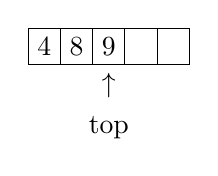
\begin{tikzpicture}[start chain=1 going right, node distance=-0.15mm]
			\node[draw, on chain=1] (a) {4};
			\node[draw, on chain=1] (b) {8};
			\node[draw, on chain=1] (c) {9};
			\node[draw, on chain=1] (d) {\phantom{0}};
			\node[draw, on chain=1] (e) {\phantom{0}};
			\node[below =of c] (top) {$\uparrow$};
				\node[below =of top] {top};
		\end{tikzpicture}
		{\caption*{Initial stack}}
	\end{subfigure}
	$\rightarrow$
	\begin{subfigure}{.3\textwidth}
		\centering
		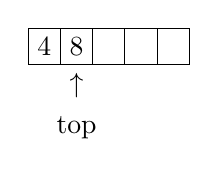
\begin{tikzpicture}[start chain=1 going right, node distance=-0.15mm]
			\node[draw, on chain=1] (a) {4};
			\node[draw, on chain=1] (b) {8};
			\node[draw, on chain=1] (c) {\phantom{0}};
			\node[draw, on chain=1] (d) {\phantom{0}};
			\node[draw, on chain=1] (e) {\phantom{0}};
			\node[below =of b] (top) {$\uparrow$};
				\node[below =of top] {top};
		\end{tikzpicture}
		{\caption*{Pop() = 9}}
	\end{subfigure}
	$\rightarrow$
	\begin{subfigure}{.3\textwidth}
		\centering
		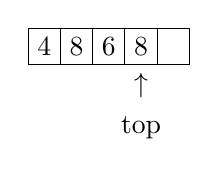
\begin{tikzpicture}[start chain=1 going right, node distance=-0.15mm]
			\node[draw, on chain=1] (a) {4};
			\node[draw, on chain=1] (b) {8};
			\node[draw, on chain=1] (c) {6};
			\node[draw, on chain=1] (d) {8};
			\node[draw, on chain=1] (e) {\phantom{0}};
			\node[below =of d] (top) {$\uparrow$};
				\node[below =of top] {top};
		\end{tikzpicture}
		{\caption*{Push(6); Push(8)}}
	\end{subfigure}
\end{figure}


%-----------------------------------------------------------------------------------------------------------------

\subsection{Queues}
\marginnote{\scriptsize{CLRS pg.232}}
A Queue is a dynamic set of data. It follows a {\bf First-In First-Out} ordering system. Imagine a checkout at a store, you enter at the end of the queue and only leave at the front. To maximize memory use, queues are sometimes implemented cicular in nature. {\bf Used as} priority queues, where elements are added with a priority and removed in order of their priority. Dijkstra's Algoirthm and A* use priority queues to track the most efficient ways to solve their problem. {\bf Insert/Delete}: $O(1)$.
\\ \\
{\bf Method:} The data structure uses {\bf Enqueue} to insert new data and {\bf Dequeue} to remove data. It uses a {\bf Head} and {\bf Tail} pointer to keep track of the data structures position in memory.

\begin{lstlisting}[style=pseudo]
Enqueue(x){
	Q[Q.tail] = x
	if Q.tail == Q.length
		Q.tail = 1
	return Q.tail = Q.tail + 1
}
Dequeue(){
	x = Q[Q.head]
	if Q.head == Q.length
		Q.head = 1
	else
		Q.head = Q.head + 1
	return x
}
\end{lstlisting}

\begin{figure}[h]
	\centering
	\begin{subfigure}{.3\textwidth}
		\centering
		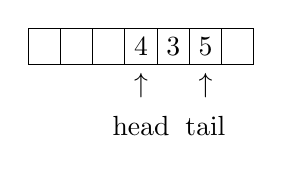
\begin{tikzpicture}[start chain=1 going right, node distance=-0.15mm]
			\node[draw, on chain=1] (f) {\phantom{0}};
			\node[draw, on chain=1] (g) {\phantom{0}};
			\node[draw, on chain=1] (a) {\phantom{0}};
			\node[draw, on chain=1] (b) {4};
			\node[draw, on chain=1] (c) {3};
			\node[draw, on chain=1] (d) {5};
			\node[draw, on chain=1] (e) {\phantom{0}};
			\node[below =of b] (head) {$\uparrow$};
				\node[below =of head] {head};
			\node[below =of d] (tail) {$\uparrow$};
				\node[below =of tail] {tail};
		\end{tikzpicture}
		{\caption*{Initial queue}}
	\end{subfigure}
	$\rightarrow$
	\begin{subfigure}{.3\textwidth}
		\centering
		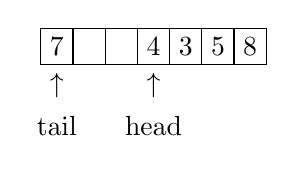
\begin{tikzpicture}[start chain=1 going right, node distance=-0.15mm]
			\node[draw, on chain=1] (f) {7};
			\node[draw, on chain=1] (g) {\phantom{0}};
			\node[draw, on chain=1] (a) {\phantom{0}};
			\node[draw, on chain=1] (b) {4};
			\node[draw, on chain=1] (c) {3};
			\node[draw, on chain=1] (d) {5};
			\node[draw, on chain=1] (e) {8};
			\node[below =of b] (head) {$\uparrow$};
				\node[below =of head] {head};
			\node[below =of f] (tail) {$\uparrow$};
				\node[below =of tail] {tail};
		\end{tikzpicture}
		{\caption*{Enqueue(8); Enqueue(7)}}
	\end{subfigure}
	$\rightarrow$
	\begin{subfigure}{.3\textwidth}
		\centering
		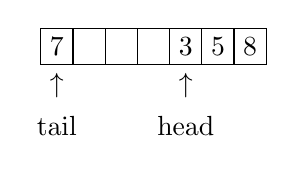
\begin{tikzpicture}[start chain=1 going right, node distance=-0.15mm]
			\node[draw, on chain=1] (f) {7};
			\node[draw, on chain=1] (g) {\phantom{0}};
			\node[draw, on chain=1] (a) {\phantom{0}};
			\node[draw, on chain=1] (b) {\phantom{0}};
			\node[draw, on chain=1] (c) {3};
			\node[draw, on chain=1] (d) {5};
			\node[draw, on chain=1] (e) {8};
			\node[below =of c] (head) {$\uparrow$};
				\node[below =of head] {head};
			\node[below =of f] (tail) {$\uparrow$};
				\node[below =of tail] {tail};
		\end{tikzpicture}
		{\caption*{Dequeue() = 4}}
	\end{subfigure}
\end{figure}


%-----------------------------------------------------------------------------------------------------------------

\subsection{Linked Lists}
\marginnote{\scriptsize{CLRS pg.236}}
In Linked Lists data is stored linearly and sequenitially. Each node contains a pointer to the next node in the list. In a {\bf Double Linked List} each node also has a pointer to it's parent. Better then dynamic arrays for inserts/deletes and since it uses pointers, the data structure can be spread across memory. However, you can not random access a linked list, in order to get an element you must transverse the list to get there. Linked lists use slightly more memory per node to track the pointers. {\bf Search:} $O(n)$; {\bf Insert/Delete}: $O(1)$.

\begin{wrapfigure}{r}{7cm}
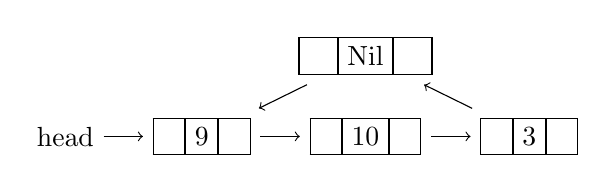
\begin{tikzpicture}[node distance=0.3cm and 0.5cm]
	\node (null)               {\fbox{\phantom{N}}\fbox{Nil}\fbox{\phantom{N}}};
	\node[below =of null] (e1) {\fbox{\phantom{0}}\fbox{10}\fbox{\phantom{0}}};
	\node[left =of e1] (e0)    {\fbox{\phantom{0}}\fbox{9}\fbox{\phantom{0}}};
	\node[right =of e1] (e2)   {\fbox{\phantom{0}}\fbox{3}\fbox{\phantom{0}}};
	\node[left =of e0] (head) {head};
	\foreach \from/\to in {null/e0, e0/e1,e1/e2,e2/null, head/e0}
		\draw[->] (\from) -- (\to);
\end{tikzpicture}
\end{wrapfigure}

\begin{lstlisting}[style=pseudo]
Search(k){
	x = L.head
	while x != Nil && x.key != k
		x = x.next
	return x
}
Insert(x){
	x.next = L.head
	if L.head != Nil
		L.head.prev = x
	L.head = x
	x.prev = Nil
}
Delete(x){
	x.prev.next = x.next
	x.next.prev = x.prev
}
\end{lstlisting}



%-----------------------------------------------------------------------------------------------------------------

\subsection{Heaps}
\marginnote{\scriptsize{CLRS pg.151}}
Heaps are a data structure which create a tree-like structure using sequential memory. They are defined by a {\bf Heap Property} which dictate how the heap is formed, eg. max-heap property: Parent nodes are always larger then their children. The internal structure of a heap may be largely unordered, but the heap property ensures the top of the heap is the max element of the data structure. Heaps are useful for any scenerio where simply knowing the largest element is needed, eg. {\bf Priority Queues}. Using properties of sequiential access, node navigation can be done using math on the node's index.
\\ \\
{\bf Method:} Heapify ensures that the node at the given index is following the heap property, if not it will "float down" the data structure until it does. When extracting the max value from a heap, replace it with the last value in the heap, and Heapify from the top.

\begin{wrapfigure}{r}{4cm}
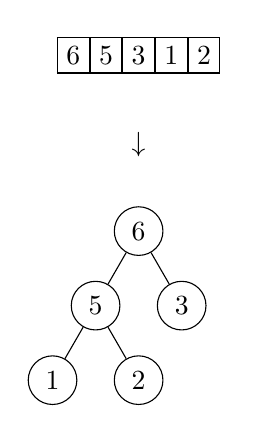
\begin{tikzpicture}[node distance=0.5cm and 0.1cm]
	\node (s) {\fbox{6}\fbox{5}\fbox{3}\fbox{1}\fbox{2}};
	\node[below =of s] (arrow) {$\downarrow$};
	\node[below =of arrow, circle, draw] (a) {6};
		\node[below left  =of a, circle, draw] (b) {5};
		\node[below right =of a, circle, draw] (c) {3};
		\node[below left  =of b, circle, draw] (d) {1};
		\node[below right =of b, circle, draw] (e) {2};
	\foreach \from/\to in {a/b,a/c,b/d,b/e}
		\draw (\from) -- (\to);
\end{tikzpicture}
\end{wrapfigure}

\begin{lstlisting}[style=pseudo]
Parent(i) => floor(i/2)
Left(i) => 2i
Right(i) => 2i + 1

BuildHeap(A){
	for i = floor(A.length/2) -> 1
		Heapify(A, i)
}
Heapify(A, i){
	if A[Left(i)] > A[i]
		largest = Left(i)
	else
		largest = i
	if A[Right(i)] > A[largest]
		largest = Right(i)
	if largest != i
		swap A[i] with A[largest]
		Heapify(A, largest)
}
Extract(A){
	max = A[0]
	A[0] = A[A.length]
	Heapify(A,0)
	return max
}
\end{lstlisting}


%-----------------------------------------------------------------------------------------------------------------

\subsection{Hashtables}
\marginnote{\scriptsize{CLRS pg.257}}
Hashtables is a data structure that map keys to values in an associated array using a {\bf Hash Function}. A hash function maps the value to the address space of the data structure. It should be choosen that limits clumping and collisions. A hash table's {\bf Load Factor} is the ratio of the number of elements in the data structure against it maximum size. When a hash table has a high load factor it has to be resized in order to avoid collisions. {\bf Search/Insert/Delete:} $O(1)$.
\\ \\
Collisions resolution could be done one of three ways: {\bf Chaining}, {\bf Open Addressing}, {\bf Cuckoo}
\begin{description}
	\item[Chaining] Each entry in the hash table is a linked list which stores all the collisions for that hash value.
	\item[Open Addressing] A probe sequence is used to check for values in a specific order. Performace degrades after a load factor above 0.7 and hash function must be very uniformly distributed.
	\item[Cuckoo] Assures constant lookup time in the worst case. Uses multiple hash functions, whenever there is a collision, it uses the next hash function to store the value. Extremely good at utilizing space.
\end{description}
There are two main methods for {\bf resizing} a hashtable:
\begin{enumerate}
	\item {\bf Rehash}: A new table size is allocated and every entry is copied over using the new hash function.
	\item {\bf Incremental}: Create a new table of the larger size, keeping the old table. Perform lookups and deletes on both tables. Whenever you insert, only insert into the new table, as well as copy over a number of element from the old table. When all elements are moved over, delete the old table.
\end{enumerate}
A technique to speed up deletes is to use {\bf Tombstones}. A tombstone is a special entry that is inserted in place of an element you wish to delete. It's ignored during lookups, and replaced during inserts.


\clearpage
\subsection{Problems}
	\begin{enumerate}
		\item Implement an algorithm to determine if a string has all unique characters. What if you cannot use additional data structures
		\item Given two strings, write a method to decide if one is a permutation of the other.
		\item Given an image represented by an NxN matrix, where each pixel in the image is 4 bytes, write a method to rotate the image by 90 degrees. Can you do this in place?
		\item Write an algorithm such that if an element in an MxN matrix is 0, its entire row and column are set to 0.
		\item Implement an algorithm to find the kth to last element of a singly linked list.
		\item Write code to partition a linked list around a value x, such that all nodes less than x come before all nodes greater than or equal to x.
		\item Implement a function to check if a linked list is a palindrome
		\item Implement a queue class which implements a queue using two stacks.
		\item Write a program to sort a stack in ascending order (with biggest items on top). You may use at most one additional stack to hold items, but you may not copy the elements into any other data structure (such as an array). The stack supports the following operations: \texttt{push}, \texttt{pop}, \texttt{peek}, and \texttt{isEmpty}.
	\end{enumerate}




\clearpage
\section{Sorting}

%-----------------------------------------------------------------------------------------------------------------

\subsection{MergeSort}
\marginnote{\scriptsize{CLRS pg.31}}
MergeSort is a {\bf Divide and Conquer algorithm}, it's recursive and can be parallelized well between multiple processors. It has {\bf Stable Sorting}, so items with the same value perserve their order from the original list. {\bf Avg/Worst Case}: $O(n \log n)$; {\bf Aux. Space}: $\Omega(n)$. {\bf Best used} when accessing data sequentially is important, eg. parallel/external sorting. On average slower then HeapSort and QuickSort.
\\ \\
{\bf Method:} MergeSort splits its list until it's down to 1 element, then rejoins them recursively inorder.

\begin{wrapfigure}{r}{2cm}
	\begin{tikzpicture}
	[scale=1.0, transform canvas={scale=1.0},
	node distance=0.2cm and 0.07cm,
	every node/.style={align=center}]
	\node (s0) {\fbox{6}\fbox{2}\fbox{1}\fbox{5}};
	\node[below left=of s0] (s1a) {\fbox{6}\fbox{2}};
	\node[below right=of s0] (s1b) {\fbox{1}\fbox{5}};
	\node[below left=of s1a] (s2a) {\fbox{6}};
	\node[below right=of s1a] (s2b) {\fbox{2}};
	\node[below left=of s1b] (s2c) {\fbox{1}};
	\node[below right=of s1b] (s2d) {\fbox{5}};
	\node[below right=of s2a] (s3a) {\fbox{2}\fbox{6}};
	\node[below left=of s2d] (s3b) {\fbox{1}\fbox{5}};
	\node[below left=of s3b] (s4) {\fbox{1}\fbox{2}\fbox{5}\fbox{6}};
	\foreach \from/\to in {
		s0/s1a,s0/s1b,
		s1a/s2a,s1a/s2b,s1b/s2c,s1b/s2d,
		s2a/s3a,s2b/s3a,s2c/s3b,s2d/s3b,
		s3a/s4,s3b/s4}
		\draw[->] (\from) -- (\to);
	\end{tikzpicture}
\end{wrapfigure}
\begin{lstlisting}[style=pseudo]
MergeSort(list){
	if length(list) <= 1
		return list
	split list -> A, B
	A = MergeSort(A), B = MergeSort(B)
	loop through each A, B and merge in sorted order
	return result
}
\end{lstlisting}
\vspace{10 mm}

%-----------------------------------------------------------------------------------------------------------------

\subsection{QuickSort}
\marginnote{\scriptsize{CLRS pg.170}}
QuickSort is a {\bf Divide and Conquer algorithm}, it's recursive and can be parallelized well between multiple processors. It has {\bf Non-Stable Sorting}, so items with the same value do not perserve their order from the original list. {\bf Avg Case}: $O(n \log n)$; {\bf Worst Case}: $O(n^2)$; {\bf Aux. Space}: $\Omega(\log n)$. {\bf Best used} when speed is top priority. Can have cases where running time is very slow, bad for very large data sets and possible for attacks.
\\ \\
{\bf Method:} QuickSort chooses a pivot, then creates two new lists, one containing elements less then the pivot and one greater then the pivot. Recursively applies this to the new lists. Rejoins them with the pivot.


\begin{wrapfigure}{r}{2cm}
\begin{tikzpicture}
[scale=1.0,
transform canvas={scale=1.0},
node distance=0.2cm and 0.04cm,
every node/.style={align=center}]
\node (s0) {\fbox{5}\fbox{2}\thickbox{3}\fbox{1}\fbox{6}};
\node[below left=of  s0] (s1a) {\thickbox{2}\fbox{1}};
\node[below right=of s0] (s1c) {\thickbox{5}\fbox{6}};

\node[below left=of  s1a] (s2a) {\fbox{1}};
\node[below =of      s1a] (s2b) {\thickbox{2}};
\node[below right=of s1a] (s2c) {\fbox{\phantom{0}}};

\node[below left=of  s1c] (s2d) {\fbox{\phantom{0}}};
\node[below =of      s1c] (s2e) {\thickbox{5}};
\node[below right=of s1c] (s2f) {\fbox{6}};

\node[below =of s2c] (s3a) {\fbox{1}\fbox{2}};
\node[yshift=-2.85cm] (s3b) {\thickbox{3}};
\node[below =of s2d] (s3c) {\fbox{5}\fbox{6}};

\node[below =of s3b] (s4) {\fbox{1}\fbox{2}\fbox{3}\fbox{5}\fbox{6}};

\foreach \from/\to in {
	s0/s1a,s0/s1c,
	s1a/s2a,s1a/s2b,s1a/s2c,  s1c/s2d,s1c/s2e,s1c/s2f,
	s2a/s3a,s2b/s3a,s2c/s3a,  s0/s3b,  s2d/s3c,s2e/s3c,s2f/s3c,
	s3a/s4, s3b/s4, s3c/s4}
	\draw[->] (\from) -- (\to);
\end{tikzpicture}
\end{wrapfigure}

\begin{lstlisting}[style=pseudo]
QuickSort(list){
	if length(list) <= 1
		return list
	select and remove a pivot  from list
	create empty lists -> left, right
	for each x in array
		if x <= pivot
			append x to left
		else
			append x to right
	return join(QuickSort(left), pivot, QuickSort(right))
}
\end{lstlisting}


%-----------------------------------------------------------------------------------------------------------------
\clearpage
\subsection{HeapSort}
\marginnote{\scriptsize{CLRS pg.151}}

Heapsort is a comparison-based sorting algorithm. It has {\bf Non-Stable Sorting}, so items with the same value do not perserve their order from the original list. {\bf Avg/Worst Case}: $O(n \log n)$; {\bf Aux. Space}: $\Omega(1)$. {\bf Best used} when space is a concerned, eg. embedded systems. On average runs slower then QuickSort, but faster then MergeSort.
\\ \\
{\bf Method:} HeapSort first builds a heap out of the data, the iteratively removes the largest elements from the heap and stores it in an array, then rebuilds the heap. Repeat until the heap is exhausted.
\begin{lstlisting}[style=pseudo]
HeapSort(A){
	BuildHeap(A)
	for length(A)
		result = Extract(A)
		replace with last in heap
		reduce heap size by 1
		Heapify(A)
	return result
}
\end{lstlisting}




\begin{figure}[h]
	\centering
	\begin{subfigure}{.3\textwidth}
		\centering
		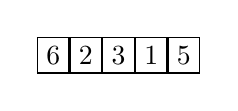
\begin{tikzpicture}[node distance=0.5cm and 0.1cm]
			\node (s) {\fbox{6}\fbox{2}\fbox{3}\fbox{1}\fbox{5}};
			%\node[below =of s, circle, draw] (a) {\phantom{0}};
				%\node[below left  =of a, circle, draw] (b) {\phantom{0}};
				%\node[below right =of a, circle, draw] (c) {\phantom{0}};
				%\node[below left  =of b, circle, draw] (d) {\phantom{0}};
				%\node[below right =of b, circle, draw] (e) {\phantom{0}};
			%\foreach \from/\to in {a/b,a/c,b/d,b/e}
				%\draw (\from) -- (\to);
		\end{tikzpicture}
		{\caption*{Initial array}}
	\end{subfigure}
	$\rightarrow$
	\begin{subfigure}{.3\textwidth}
		\centering
		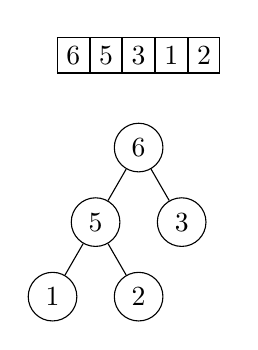
\begin{tikzpicture}[node distance=0.5cm and 0.1cm]
			\node (s) {\fbox{6}\fbox{5}\fbox{3}\fbox{1}\fbox{2}};
			\node[below =of s, circle, draw] (a) {6};
				\node[below left  =of a, circle, draw] (b) {5};
				\node[below right =of a, circle, draw] (c) {3};
				\node[below left  =of b, circle, draw] (d) {1};
				\node[below right =of b, circle, draw] (e) {2};
			\foreach \from/\to in {a/b,a/c,b/d,b/e}
				\draw (\from) -- (\to);
		\end{tikzpicture}
		{\caption*{Reorganized as a heap}}
	\end{subfigure}
	$\rightarrow$
	\begin{subfigure}{.3\textwidth}
		\centering
		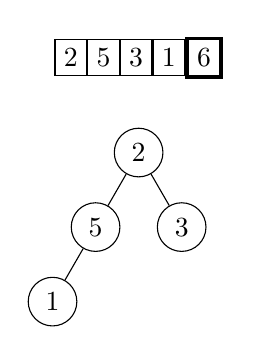
\begin{tikzpicture}[node distance=0.5cm and 0.1cm]
			\node (s) {\fbox{2}\fbox{5}\fbox{3}\fbox{1}\thickbox{6}};
			\node[below =of s, circle, draw] (a) {2};
				\node[below left  =of a, circle, draw] (b) {5};
				\node[below right =of a, circle, draw] (c) {3};
				\node[below left  =of b, circle, draw] (d) {1};
			\foreach \from/\to in {a/b,a/c,b/d}
				\draw (\from) -- (\to);
		\end{tikzpicture}
		{\caption*{Remove root node, \par replaced with last}}
	\end{subfigure}
\end{figure}


\begin{figure}[h]
	\centering
	\begin{subfigure}{.3\textwidth}
		\centering
		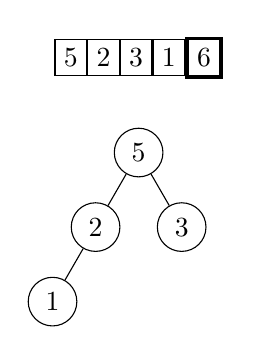
\begin{tikzpicture}[node distance=0.5cm and 0.1cm]
			\node (s) {\fbox{5}\fbox{2}\fbox{3}\fbox{1}\thickbox{6}};
			\node[below =of s, circle, draw] (a) {5};
				\node[below left  =of a, circle, draw] (b) {2};
				\node[below right =of a, circle, draw] (c) {3};
				\node[below left  =of b, circle, draw] (d) {1};
			\foreach \from/\to in {a/b,a/c,b/d}
				\draw (\from) -- (\to);
		\end{tikzpicture}
		{\caption*{Heapify}}
	\end{subfigure}
	$\rightarrow$
	\begin{subfigure}{.3\textwidth}
		\centering
		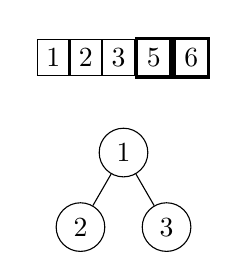
\begin{tikzpicture}[node distance=0.5cm and 0.1cm]
			\node (s) {\fbox{1}\fbox{2}\fbox{3}\thickbox{5}\thickbox{6}};
			\node[below =of s, circle, draw] (a) {1};
				\node[below left  =of a, circle, draw] (b) {2};
				\node[below right =of a, circle, draw] (c) {3};
			\foreach \from/\to in {a/b,a/c}
				\draw (\from) -- (\to);
		\end{tikzpicture}
		{\caption*{Remove root node, \par replaced with last}}
	\end{subfigure}
	$\rightarrow$
	\begin{subfigure}{.3\textwidth}
		\centering
		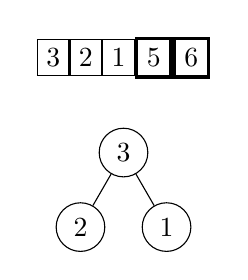
\begin{tikzpicture}[node distance=0.5cm and 0.1cm]
			\node (s) {\fbox{3}\fbox{2}\fbox{1}\thickbox{5}\thickbox{6}};
			\node[below =of s, circle, draw] (a) {3};
				\node[below left  =of a, circle, draw] (b) {2};
				\node[below right =of a, circle, draw] (c) {1};
			\foreach \from/\to in {a/b,a/c}
				\draw (\from) -- (\to);
		\end{tikzpicture}
		{\caption*{Re-heapify!}}
	\end{subfigure}
	{\caption*{Example of heaping an array}}
\end{figure}


\clearpage
	\subsection{Problems}
		\begin{enumerate}
			\item Write a method to sort an array of strings so that all the anagrams are next to each other.
			\item Imagine you have a 20 GB file with one string per line. Explain how you would sort the file.
			\item Given an M x N matrix in which each row and each column is sorted in ascending order, write a method to find an element.
			\item A circus is designing a tower routine consisting of people standing atop one another's shoulders. For practical and aesthetic reasons, each person must be both shorter and lighter than the person below him or her. Given the heights and weights of each person in the circus, write a method to compute the largest possible number of people in such a tower.
				\begin{lstlisting}[style=pseudo]
	Example
	Input (ht,wt): (65, 100) (70, 150) (56, 90) (75, 190) (60, 95) (68, 110)
	Output:The longest tower is (56, 90) (60,95) (65,100) (68,110) (70,150) (75,190)
				\end{lstlisting}
		\end{enumerate}


\clearpage
\section{Trees}
%-----------------------------------------------------------------------------------------------------------------

\subsection{Binary Search Trees}
\marginnote{\scriptsize{CLRS pg.287}}
Binary Trees are family of data structures efficient at lookups. Data is stored that $Right \leq Node \leq Left$. BSTs are {\bf unbalanced}, meaning one part of the tree may become much larger then the other, hurting the efficiency. {\bf Search/Insert:} $O(n \log n)$; {\bf Delete:} $O(n)$.

%\begin{lstlisting}[style=pseudo]
%Search(node, val){
	%if node == Nil or node.key == val
		%return node
	%if val > node.key
		%return Search(node.left, val)
	%else
		%return Search(node.right, val)
%}
%Insert(node, val){
	%if node is empty
		%node = val
%
	%if val > .key
			%x = x.left
		%else
			%x = x.right
	%if val > x.parent.key
		%x.left = val
	%else
		%x.right = val
%}
%Delete(T, node){
	%if node.left == Nil and node.right == Nil
	%//TODO
%}
%\end{lstlisting}

\begin{figure}[h]
	\centering
	\begin{subfigure}{.4\textwidth}
		\centering
		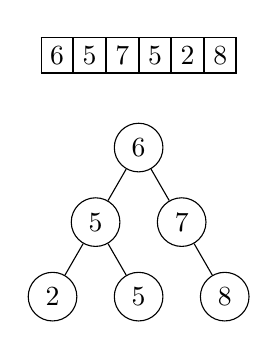
\begin{tikzpicture}[node distance=0.5cm and 0.1cm]
			\node (s) {\fbox{6}\fbox{5}\fbox{7}\fbox{5}\fbox{2}\fbox{8}};
			\node[below =of s, circle, draw] (a) {6};
				\node[below left  =of a, circle, draw] (b) {5};
				\node[below right =of a, circle, draw] (c) {7};
				\node[below left  =of b, circle, draw] (d) {2};
				\node[below right =of b, circle, draw] (e) {5};
				\node[below right =of c, circle, draw] (f) {8};
			\foreach \from/\to in {a/b,a/c,b/d,b/e,c/f}
				\draw (\from) -- (\to);
		\end{tikzpicture}
		{\caption*{Well-balanced BST}}
	\end{subfigure}
	\begin{subfigure}{.4\textwidth}
		\centering
		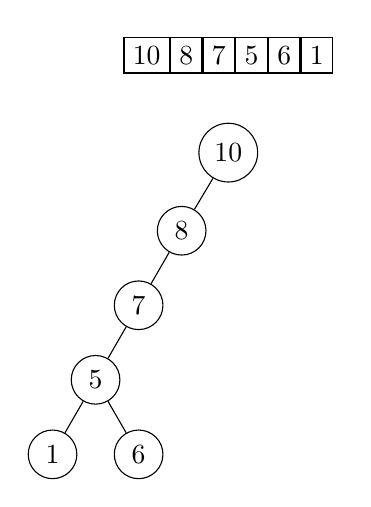
\begin{tikzpicture}[node distance=0.5cm and 0.1cm]
			\node (s) {\fbox{10}\fbox{8}\fbox{7}\fbox{5}\fbox{6}\fbox{1}};
			\node[below =of s, circle, draw] (a) {10};
				\node[below left  =of a, circle, draw] (b) {8};
				\node[below left  =of b, circle, draw] (c) {7};
				\node[below left  =of c, circle, draw] (d) {5};
				\node[below left  =of d, circle, draw] (e) {1};
				\node[below right =of d, circle, draw] (f) {6};
			\foreach \from/\to in {a/b,b/c,c/d,d/e,d/f}
				\draw (\from) -- (\to);
		\end{tikzpicture}
		{\caption*{Unbalanced BST}}
	\end{subfigure}
\end{figure}

%-----------------------------------------------------------------------------------------------------------------

\subsection{B-Trees}
\marginnote{\scriptsize{CLRS pg.488}}
B-Trees are an extreme form of {\bf k-ary Trees}, where k is very large. Each node has a minimum and maximum number of children it can have; $t-1$ and $2t - 1$ respectively, where $t$ is the {\bf order} of the tree. B-Trees are achieve extremely large tree structures with a small height when the order of the tree is high, number of nodes is $2t^h -1$ where $h$ is the height of the tree. {\bf Search/Insert/Delete:} $O(\log n)$.
\\ \\
{\bf Best Used} for when lookups are very expensive and when lookups are best done in large sequiential blocks. Mostly used for storing data on {\bf physical storage}.

\begin{figure}[h]
	\centering
	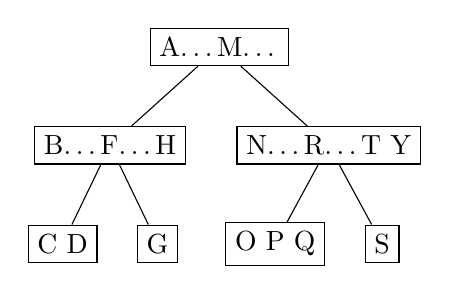
\begin{tikzpicture}[every tree node/.style={draw},
		level distance=1.25cm,sibling distance=.5cm,
		edge from parent path={(\tikzparentnode) -- (\tikzchildnode)}]
		\Tree [.{A\ldots M\ldots}
			[.{B\ldots F\ldots H}
				[.{C D} ]
				[.{G} ]
			]
			[.{N\ldots R\ldots T Y}
				[.{O P Q} ]
				[.{S} ]
			]
		]
	\end{tikzpicture}
	{\caption*{B-tree with order of 2}}
\end{figure}
Inserting a node is slightly more complicated. When inserting a new value into a node that is full, we must split the node into smaller chunks. With deleting a value, you may have to rearrange a node's children.
\begin{figure}[h]
	\centering
	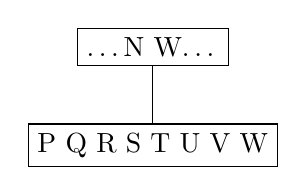
\begin{tikzpicture}[every tree node/.style={draw},
		level distance=1.25cm,sibling distance=.5cm,
		edge from parent path={(\tikzparentnode) -- (\tikzchildnode)}]
		\Tree [.{\ldots N W\ldots}
			[.{P Q R S T U V W} ]
		]
	\end{tikzpicture}
	\hspace{1 cm} \raisebox{1.0cm}{$\rightarrow$} \hspace{1 cm}
	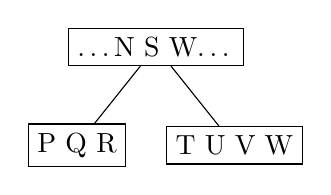
\begin{tikzpicture}[every tree node/.style={draw},
		level distance=1.25cm,sibling distance=.5cm,
		edge from parent path={(\tikzparentnode) -- (\tikzchildnode)}]
		\Tree [.{\ldots N S W\ldots}
			[.{P Q R} ]
			[.{T U V W} ]
		]
	\end{tikzpicture}
	{\caption*{Splitting a child node into 2 on $S$ because it is too large}}
\end{figure}


%-----------------------------------------------------------------------------------------------------------------

\subsection{Tries}
A Trie is an unique tree data structure where a node's location within the tree determines its value. Each edge of the tree has a value given to it and as you traverse the tree you build the value of the node. Very useful for {\bf storing strings} and {\bf binary values}.
\\ \\
Tries have a {\bf faster worst case than hash tables} because they don't need to rebuilds, they can produce {\bf alpha-ordering} which may be useful for some applications like spell checking, and there is {\bf no chance for collisions}. However, Tries may need more memory, long entires can create useless nodes, and they require {\bf lots of random access memory} to operate. {\bf Search/Insert/Delete:} $O(k)$ where $k$ is the length of the longest node value.

\begin{figure}[h]
	\centering
	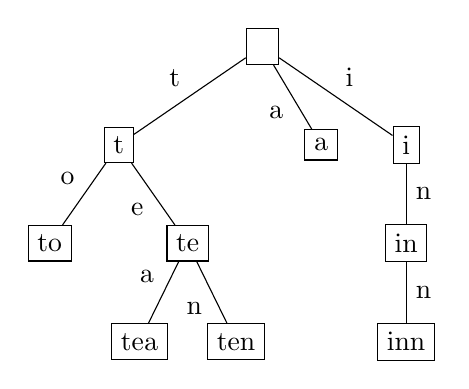
\begin{tikzpicture}[every tree node/.style={draw},
		level distance=1.25cm,sibling distance=.5cm,
		edge from parent path={(\tikzparentnode) -- (\tikzchildnode)}]
		\Tree [.\phantom{0}
			\edge node[auto=right] {t};
			[.t
				\edge node[auto=right] {o};
				[.to ]
				\edge node[auto=right] {e};
				[.te
					\edge node[auto=right] {a};
					[.tea ]
					\edge node[auto=right] {n};
					[.ten ]
				]
			]
			\edge node[auto=right] {a};
			[.a ]
			\edge node[auto=left] {i};
			[.i
				\edge node[auto=left] {n};
				[.in
					\edge node[auto=left] {n};
					[.inn ]
				]
			]
		]
	\end{tikzpicture}
	{\caption*{Building a Trie for "to", "tea", "ten", and "inn"}}
\end{figure}


%-----------------------------------------------------------------------------------------------------------------

\subsection{Radix Tree}
\marginnote{\scriptsize{CLRS pg.304}}
Radix Tress are space optimized {\bf Trie} where each node with only one child is merged with its parent, and its edge is updated accordingly. They are {\bf more efficient for small sets} especially if the strings are long and for sets of strings that share long prefixes. {\bf Search/Insert/Delete:} $O(k)$ where $k$ is the length of the longest edge key.
\\ \\
{\bf Best used} in IP Routing, where the ability to contain large ranges of values with a few exceptions is particularly suited to the hierarchical organization of IP addresses. They are useful for {\bf Inverted Indexes} in text documents for very fast searching through the document.

\begin{figure}[h]
	\centering
	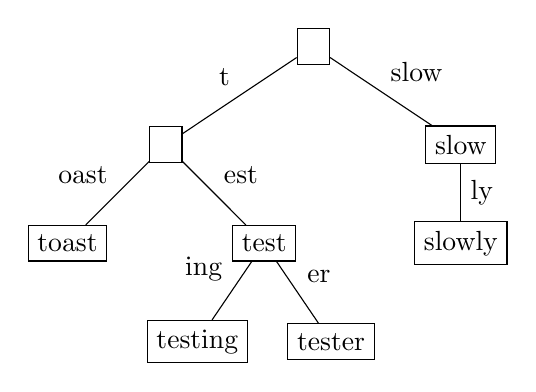
\begin{tikzpicture}[every tree node/.style={draw},
		level distance=1.25cm,sibling distance=.5cm,
		edge from parent path={(\tikzparentnode) -- (\tikzchildnode)}]
		\Tree [.\phantom{0}
			\edge node[auto=right] {t};
			[.\phantom{0}
				\edge node[auto=right] {oast};
				[.toast ]
				\edge node[auto=left] {est};
				[.test
					\edge node[auto=right] {ing};
					[.testing ]
					\edge node[auto=left] {er};
					[.tester ]
				]
			]
			\edge node[auto=left] {slow};
			[.slow
				\edge node[auto=left] {ly};
				[.slowly ]
			]
		]
	\end{tikzpicture}
	{\caption*{Building a Radix Trie for "toast", "test", "testing", "tester", "slow", and "slowly"}}
\end{figure}


%-----------------------------------------------------------------------------------------------------------------

\subsection{Self-Balancing Trees}
\marginnote{\scriptsize{CLRS pg.308}}
A Self-Balancing Tree is a binary search tree that keeps its height small during inserts and deletes. Binary Search Trees have a very bad worst-case; Self-Balancing Trees attempt to correct this by using {\bf Tree Rotations} to maintain tree properties that ensure a predictable height of the tree.
\\ \\
Whenever a node is inserted or deleted, we need to check the node's children for consistency of the height property. {\bf Avg/Worst} of {\bf Search/Insert/Deletes:}$O(\log n)$. The two most common Self-Balancing Trees are {\bf AVL Trees} and {\bf Red-Black Trees}.

\begin{figure}[h]
	\centering
	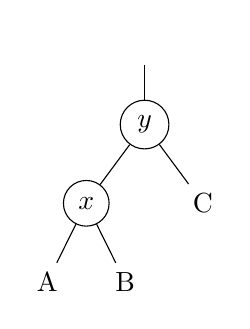
\begin{tikzpicture}[
			every tree node/.style={},
			level distance=1.0cm,sibling distance=.5cm,
			edge from parent path={(\tikzparentnode) -- (\tikzchildnode)}
		]
		\Tree [.\phantom{0}
			[.\node[draw, circle] {$y$};
				[.\node[draw, circle] {$x$};
					[.A ]
					[.B ]
				]
				[.C ]
			]
		]
	\end{tikzpicture}
	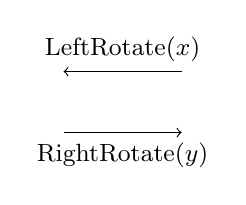
\begin{tikzpicture}[node distance=0.3cm and 1.5cm]
		\node                (tl) {\phantom{0}};
		\node [right =of tl] (tr) {\phantom{0}};
		\node [below =of tl] (bl) {\phantom{0}};
		\node [right =of bl] (br) {\phantom{0}};
		\draw[->] (tr) --(tl) node[above,midway] {\small LeftRotate($x$)};
		\draw[->] (bl) --(br) node[below,midway] {\small RightRotate($y$)};
	\end{tikzpicture}
	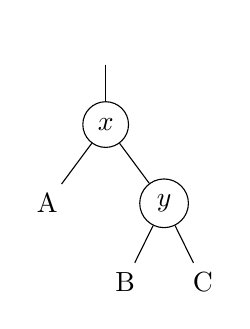
\begin{tikzpicture}[
			every tree node/.style={},
			level distance=1.0cm,sibling distance=.5cm,
			edge from parent path={(\tikzparentnode) -- (\tikzchildnode)}
		]
		\Tree [.\phantom{0}
			[.\node[draw, circle] {$x$};
				[.A ]
				[.\node[draw, circle] {$y$};
					[.B ]
					[.C ]
				]
			]
		]
	\end{tikzpicture}
	%{\caption*{Basic Tree Rotations}}
\end{figure}

%-----------------------------------------------------------------------------------------------------------------

\subsubsection{AVL Trees}
The height property of an AVL Tree is that {\bf the heights of the two child subtrees of any node differ by at most one}. AVL Trees are more rigidly balanced than Red-Black Trees, leading to {\bf slower inserts and deletes} but {\bf faster search}.

%\begin{minipage}{\linewidth}
%\begin{lstlisting}[style=pseudo]
%balanceFactor(node) => height(node.left) - height(node.right)
%Insert(node, val){
	%if node is Nil
		%node.key = val
		%return node
	%if val > node.key
		%node.left = Insert(node.left, val)
		%if balanceFactor(node) > 1
			%if val > node.left.key
				%LeftRotate(node)
			%LeftRotate(node)
	%if val <= node.key
		%node.right = Insert(node.right, val)
		%if balanceFactor(node) < -1
			%if val < node.right.key
				%RightRotate(node)
			%RightRotate(node)
	%return node
%}
%
%Delete(z){
	%//finish later, very complex
%}
%\end{lstlisting}
%\end{minipage}
%-----------------------------------------------------------------------------------------------------------------

\subsubsection{Red-Black Trees}
Red-Black Trees are less rigidly balanced than AVL Trees, leading to {\bf slower search} but {\bf faster inserts and deletes}. The height properties of a Red-Black Tree are as follows:
\begin{enumerate}
	\item A node may be red or black
	\item All leaves are black
	\item Every red node must have two black child nodes
	\item Every path from the root to a leaf must have the same number of black nodes.
\end{enumerate}

\begin{figure}[h]
\centering
\tikzset{
	node_black/.style = {
		circle, white, font=\sffamily\bfseries, draw=black, fill=black
	},
	node_red/.style = {
		circle, red, draw=red, very thick
	},
	node_nil/.style = {
		white, font=\scriptsize\sffamily\bfseries, draw=black, fill=black
	}
}
\begin{tikzpicture}[every tree node/.style={draw},
	level distance=1.25cm,sibling distance=.5cm,
	edge from parent path={(\tikzparentnode) -- (\tikzchildnode)}]
	\Tree [.\node[node_black] {13};
		[.\node[node_red] {8};
			[.\node[node_black] {1};
				[.\node[node_nil] {NIL}; ]
				[.\node[node_red] {6};
					[.\node[node_nil] {NIL}; ]
				]
			]
			[.\node[node_black] {11};
				[.\node[node_nil] {NIL}; ]
				[.\node[node_nil] {NIL}; ]
			]
		]
		[.\node[node_red] {17};
			[.\node[node_black] {15};
				[.\node[node_nil] {NIL}; ]
				[.\node[node_nil] {NIL}; ]
			]
			[.\node[node_black] {25};
				[.\node[node_red] {22};
					[.\node[node_nil] {NIL}; ]
					[.\node[node_nil] {NIL}; ]
				]
				[.\node[node_red] {27};
					[.\node[node_nil] {NIL}; ]
					[.\node[node_nil] {NIL}; ]
				]
			]
		]
	]
\end{tikzpicture}
\end{figure}

%\begin{minipage}{\linewidth}
%\begin{lstlisting}[style=pseudo]
%//TODO: Make recursive
%Insert(z){
	%find leaf where node should be attached -> y
	%z.parent = y
	%if z.key > y.key
		%y.left = z
	%else
		%y.right = z
	%z.color = red
%
	%//Maintain height property
	%while z.parent is red
		%if z.parent is a left-child
			%if z.uncle is red
				%z.parent.color = black
				%z.uncle.color = black
				%z.grandparent.color = red
				%z = z.grandparent
			%if z.uncle is black and z is a right-child
				%z = z.parent
				%LeftRotate(z)
			%if z's uncle is black and z is a left-child
				%z.parent.color = black
				%z.grandparent.color = red
				%RightRotate(z.grandparent)
		%else
			%Same as above but switch left and right rotate
	%root.color = black
%}
%Delete(z){
	%//finish later, very complex
%}
%\end{lstlisting}
%\end{minipage}




%-----------------------------------------------------------------------------------------------------------------

\subsection{Bloom Filter}
A Bloom Filter is a space efficient probalistic data structure that's used to test whether an element is in a set. False positives are possible, but {\bf false negatives} are not. An empty Bloom Filter is a bit array of $m$ bits all set to 0. Whenever you add an element to the set use $k$ hash functions and flip all the corresponing entires to 1. To test if an entry belongs to the set, simply hash it and check the corresponding bit entires. If any of them are 0 the element is not part of the set. The probability of a {\bf false positive} is $(1 - e^{-kn/m})^k$, where $n$ is the number of elements encoded in the set.
\\ \\
{\bf Used in} Chrome to detect unsafe urls from a master list, BigTable to skip unnecessary table lookups, and in url shortners.

\begin{figure}[h]
	\centering
	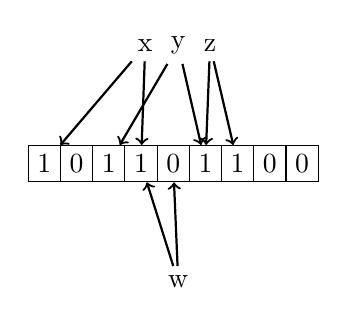
\begin{tikzpicture}[start chain=1 going right, node distance=-0.15mm]
		\node (y) {y};
		\node[left =of y] (x) {x};
		\node[right =of y] (z) {z};
		\node[draw, on chain=1] at (-1.7,-1.5) (a) {1};
		\node[draw, on chain=1] (b) {0};
		\node[draw, on chain=1] (c) {1};
		\node[draw, on chain=1] (d) {1};
		\node[draw, on chain=1] (e) {0};
		\node[draw, on chain=1] (f) {1};
		\node[draw, on chain=1] (g) {1};
		\node[draw, on chain=1] (h) {0};
		\node[draw, on chain=1] (i) {0};
		\node at (0,-3.0) (w) {w};
		\foreach \from/\to in {x/a,x/d,y/c,y/f,z/f,z/g,w/d,w/e}
			\draw[->, thick] (\from) -- (\to);
	\end{tikzpicture}
	{\caption*{$x$, $y$, $z$ are in the set, where $w$ is not}}
\end{figure}

\subsection{Problems}
	\begin{enumerate}
		\item Implement a function to check if a binary tree is balanced. For the purposes of this question, a balanced tree is defined to be a tree such that the heights of the two subtrees of any node never differ by more than one.
		\item Implement a function to check if a binary tree is a binary search tree.
		\item Write an algorithm to find the'next'node (i.e., in-order successor) of a given node in a binary search tree. You may assume that each node has a link to its parent.
		\item You are given a binary tree in which each node contains a value. Design an algorithm to print all paths which sum to a given value. The path does not need to start or end at the root or a leaf.
		\item You have two very large binary trees: Tl, with millions of nodes, and T2, with hundreds of nodes. Create an algorithm to decide if T2 is a subtree of Tl.
		\\ \\
		A tree T2 is a subtree of Tl if there exists a node n in Tl such that the subtree of n is identical to T2. That is, if you cut off the tree at node n, the two trees would be identical.
		\item Given a sorted (increasing order) array with unique integer elements, write an algorithm to create a binary search tree with minimal height.
	\end{enumerate}





\clearpage
\section{Bit Manipulation}
Bit Manipulation is the act of manipualting individual bits within data. It can reduce the need to loop over a data structure and can give many-fold speed ups, as bit manipulations are {\bf processed in parallel}, but the code can become rather more difficult to write and maintain. {\bf Used in} low-level device control, error detection and correction algorithms, data compression, encryption algorithms, and optimization.
	\subsection{Operations}
		Bit manipulation supports a number operations: OR \text{\textbar}, AND \& , XOR \string^ , SHIFT << , and NOT \string~ .
		\begin{lstlisting}[style=pseudo]
	0110 | 0001 = 0111
	1000 & 1011 = 1000
	1100 ^ 1010 = 0110
	1101 >> 2    = 0011
	~1001        = 0110
	1011 & (~0 << 2) = 1011 & 1100 = 1000
		\end{lstlisting}
		Arthemetic operations can be used.
	\begin{lstlisting}[style=pseudo]
	0110 + 0010 = 1000
	0110 - 0011 = 0101
	0011 * 0101 = 1001
	\end{lstlisting}

	\subsection{Common Tasks}
	The following are common tasks you would need to implement while manipualting bits.
	\begin{lstlisting}[style=pseudo]
//Retrieve the value of a bit at the ith position
getBit(n, i){
	return (n & (1 << i)) != 0
}
	getBit(11001101, 3)
	= (11001101 & (1 << 3)) != 0
	= (11001101 & 00001000) != 0
	= (11001101 & 00001000) != 0
	= 00001000 != 0
	= 1

//Sets the value of a bit at the ith position to 1
setBit(n, i){
	return n | (1 << i)
}
	setBit(11001101, 1)
	= 11001101 | (1 << 1)
	= 11001101 | 00000010
	= 11001111

//Sets the value of a bit at the ith position to 0
clearBit(n, i){
	return n & ~(1 << i)
}
	clearBit(11001101, 7)
	= 11001101 & ~(1 << 7)
	= 11001101 & ~(01000000)
	= 11001101 & 10111111
	= 10001101

//Sets the value of a bit at the ith position to u
updateBit(n, i, u){
	mask = ~(1 << i)
	return (n & mask) | (u << i)
}
	updateBit(11001101, 5, 1)
	= (11001101 & ~(1 << 5)) | (1 << 5)
	= (11001101 & 11011111) | 00100000
	= 11001101 | 00100000
	= 11101101
	\end{lstlisting}

	\subsection{Problems}
	\begin{enumerate}
		\item Given a positive integer, print the next smallest and the next largest number that have the same number of 1 bits in their binary representation.
		\item Explain what the following code does: \texttt{((n \& (n-1)) == 0)}.
		\item Write a program to swap odd and even bits in an integer with as few instructions as possible (e.g., bit 0 and bit 1 are swapped, bit 2 and bit 3 are swapped, and so on.
		\item Write a function that adds two numbers. You should not use any arithmetic operators.
		\item A monochrome screen is stored as a single array of bytes, allowing eight consecutive pixels to be stored in one byte.The screen has width w, where w is divisible by 8 (that is, no byte will be split across rows).The height of the screen, of course, can be derived from the length of the array and the width. Implement a function \texttt{drawHorizontalLine(byte\string[\string] screen, int width, int xl, int x2, int y)} which draws a horizontal line from (xl, y) to (x2, y).
	\end{enumerate}


\clearpage
\section{Graph Algorithms}
%-----------------------------------------------------------------------------------------------------------------
	\subsection{Representation}
	\marginnote{\scriptsize{CLRS pg.308}}
	A graph is a collection of nodes with values that are connected to eachother. {\bf Undirected Graphs} simply have links betwen two nodes, where {\bf Directed Graphs} have one-way links between nodes. We can represent a graph in one of two ways; {\bf Adjacency Lists} are useful for when the graph is {\bf sparse}, few edges compared to nodes. {\bf Adjacency Matricies} are useful for when the graph is {\bf dense}, many edges compared to nodes.
	\begin{figure}[h]
		\centering
		\begin{subfigure}[b]{.3\textwidth}
			\centering
			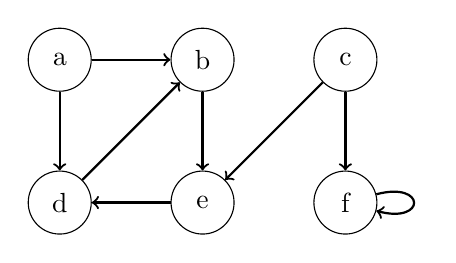
\begin{tikzpicture}[
					every node/.style={draw, circle},
					minimum size=0.8cm,
					every loop/.style={},
					node distance=1.0cm and 1.0cm]
				\node[]            (a) {a};
				\node[right =of a] (b) {b};
				\node[right =of b] (c) {c};
				\node[below =of a] (d) {d};
				\node[right =of d] (e) {e};
				\node[right =of e] (f) {f};
				\foreach \from/\to in {a/b, a/d, b/e, c/e, c/f, d/b, e/d}
					\draw[->, thick] (\from) -- (\to);
				\draw[->, thick] (f) to[loop right] (f);
			\end{tikzpicture}
			{\caption*{Directed Graph}}
		\end{subfigure}
		\begin{subfigure}[b]{.3\textwidth}
			\centering
			$a \rightarrow b,d$            \\
			$b \rightarrow e \phantom{,a}$ \\
			$c \rightarrow e,f$            \\
			$d \rightarrow b \phantom{,a}$ \\
			$e \rightarrow d \phantom{,a}$ \\
			$f \rightarrow f \phantom{,a}$
			{\caption*{Adjacency List}}
		\end{subfigure}
		\begin{subfigure}[b]{.3\textwidth}
			\centering
			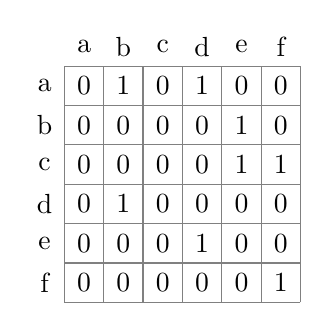
\begin{tikzpicture}
				\draw[step=0.5cm,color=gray] (-1.5,-1.5) grid (1.5,1.5);
				\foreach \v [count=\i] in {
					\phantom{0},a,b,c,d,e,f,
					a,0,1,0,1,0,0,
					b,0,0,0,0,1,0,
					c,0,0,0,0,1,1,
					d,0,1,0,0,0,0,
					e,0,0,0,1,0,0,
					f,0,0,0,0,0,1}{
				\draw let
					\n0 = 7,
					\n1 = {int(mod(\i-1,\n0))},
					\n2 = {-2.0 + 0.25 + \n1 * 0.5},
					\n3 = {2.0 + int((\i-1)/-\n0) * 0.5 - 0.25}
				in node at (\n2, \n3) {\v};
				}
			\end{tikzpicture}
			{\caption*{Adjacency Matrix}}
		\end{subfigure}
	\end{figure}


	%-----------------------------------------------------------------------------------------------------------------

	\subsection{Breadth-First Search}
	\marginnote{\scriptsize{CLRS pg.594}}
	Breadth-First Search is a strategy for searching a graph. It starts at the root node, visits all of it's neighbours, then for each neighbour, goes to their neighbours, etc. As it runs it produces a {\bf Breadth-First Tree}, where the depth of the tree indicates how far apart the root and that node is in the graph.
	\\ \\
	{\bf Worst Case:} $O(V + E)$, where $O(E)$ may vary between $O(V)$ and $O(V^2)$ depending on how dense the graph is. {\bf Aux. Space} is Adj. List:$\Omega(V + E)$ and Adj. Matrix:$\Omega(V^2)$. {\bf Used for} finding the shortest path between nodes and asserting if two nodes are connected to eachother. {\bf Useful} for when needing to find a specific node, without visitng the entire tree.

	\begin{figure}[h]
		\centering
		\begin{subfigure}[b]{.3\textwidth}
			\centering
			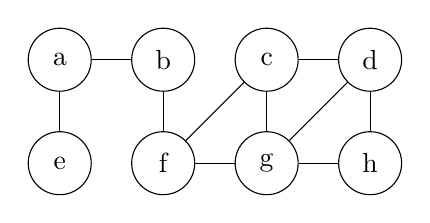
\begin{tikzpicture}[
					every node/.style={draw, circle},
					minimum size=0.8cm,
					node distance=0.5cm and 0.5cm]
				\node[]            (a) {a};
				\node[right =of a] (b) {b};
				\node[right =of b] (c) {c};
				\node[right =of c] (d) {d};

				\node[below =of a] (e) {e};
				\node[right =of e] (f) {f};
				\node[right =of f] (g) {g};
				\node[right =of g] (h) {h};
				\foreach \from/\to in {a/b, a/e, b/f, f/c, f/g, c/d, g/h,
										c/g,g/d,d/h}
					\draw (\from) -- (\to);
			\end{tikzpicture}
			{\caption*{Initial undirected graph}}
		\end{subfigure}
		\hspace{0.5cm}
		\begin{subfigure}[b]{.3\textwidth}
			\centering
			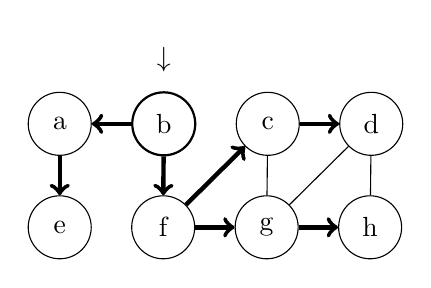
\begin{tikzpicture}[
					every node/.style={draw, circle},
					minimum size=0.8cm,
					node distance=0.5cm and 0.5cm]
				\node[]            (a) {a};
				\node[right =of a, label=above:$\downarrow$, thick] (b) {b};
				\node[right =of b] (c) {c};
				\node[right =of c] (d) {d};

				\node[below =of a] (e) {e};
				\node[right =of e] (f) {f};
				\node[right =of f] (g) {g};
				\node[right =of g] (h) {h};
				\foreach \from/\to in {b/a, a/e, b/f, f/c, f/g, c/d, g/h}
					\draw[->, ultra thick] (\from) -- (\to);
				\foreach \from/\to in {c/g,g/d,d/h}
					\draw (\from) -- (\to);
			\end{tikzpicture}
			{\caption*{BFS starting at node b}}
		\end{subfigure}
		\hspace{0.5cm}
		\begin{subfigure}[b]{.2\textwidth}
			\centering
			\begin{tikzpicture}[every tree node/.style={},
				level distance=0.75cm,sibling distance=.5cm,
				edge from parent path={(\tikzparentnode) -- (\tikzchildnode)}]
				\Tree [.b
					[.a
						[.e ]
					]
					[.f
						[.c
							[.d ]
						]
						[.g
							[.h ]
						]
					]
				]
			\end{tikzpicture}
			{\caption*{Breadth-first tree}}
		\end{subfigure}
	\end{figure}

	\begin{lstlisting}[style=pseudo]
	BFS(start, goal){
		create queue Q
		create list R
		Q.enqueue(start)
		R.push(start)

		while Q is not empty
			t = Q.dequeue()
			t.visited = true
			if t is goal
				return R
			for all neighbours v of t
				if v.visited == false
					v.visited = true
					R.push(v)
					Q.enqueue(v)
	}
	\end{lstlisting}





	%-----------------------------------------------------------------------------------------------------------------

	\subsection{Depth First Search}
	\marginnote{\scriptsize{CLRS pg.603}}
	Depth-First Search is a strategy for searching a graph. Its starts at the root node and explores as deep as possible before backtracking. By tracking and applying a {\bf timestamp} to each node as it's visited for the first and last time. You can then sort the nodes by {\bf pre-order} and {\bf post-order}, respectively. The timestamp increments when a node is visited and when its neighbours have been exhausted. Post-ordering the nodes provides you with a {\bf Topological Sort} of the graph.
	\\ \\
	{\bf Used in} AI for limiting the depth of decisions trees and evaluating branches based on heurstics, maze generation, and topological sorting. {\bf Useful} when needing to visit all nodes within a graph.


	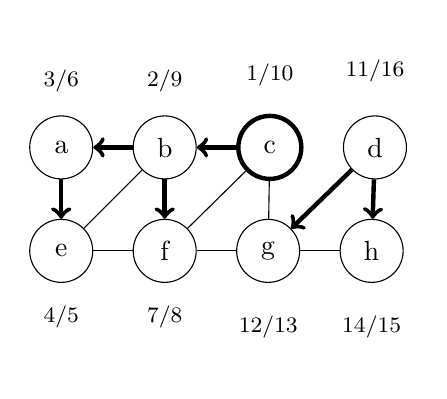
\begin{tikzpicture}[
			every node/.style={draw, circle},
			minimum size=0.8cm,
			node distance=0.5cm and 0.5cm]
		\node[             label=above:\footnotesize 3/6]   (a) {a};
		\node[right =of a, label=above:\footnotesize 2/9]   (b) {b};
		\node[right =of b, label=above:\footnotesize 1/10, ultra thick]  (c) {c};
		\node[right =of c, label=above:\footnotesize 11/16] (d) {d};

		\node[below =of a, label=below:\footnotesize 4/5]  (e) {e};
		\node[right =of e, label=below:\footnotesize 7/8]   (f) {f};
		\node[right =of f, label=below:\footnotesize 12/13] (g) {g};
		\node[right =of g, label=below:\footnotesize 14/15] (h) {h};
		\foreach \from/\to in {a/e, b/a, b/f, c/b, d/g, d/h}
			\draw[->, ultra thick] (\from) -- (\to);
		\foreach \from/\to in {c/f, e/b, f/e, g/f, g/c, h/g}
			\draw (\from) -- (\to);
	\end{tikzpicture}
	\hspace{2cm}
	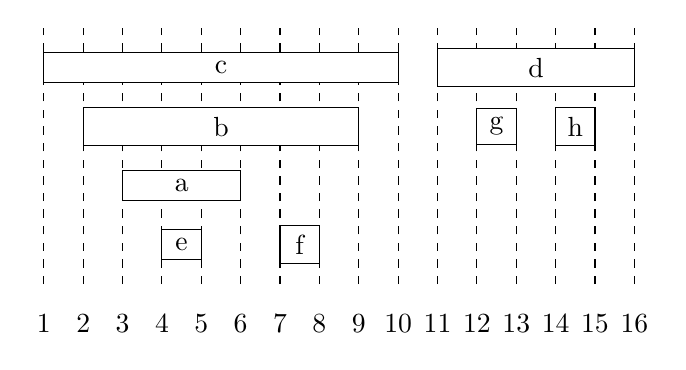
\begin{tikzpicture}[every node/.style={fill=white}]
		\foreach \i in {1,...,16} {
			\draw [dashed] (\i*0.5,1) -- (\i*.5,4.25);
			\node at (\i*0.5,0.5) {\i};
		}
		\foreach \t/\s/\e/\h in {
			a/3/6/2,
			b/2/9/1,
			c/1/10/0,
			d/11/16/0,
			e/4/5/3,
			f/7/8/3,
			g/12/13/1,
			h/14/15/1}{
			\draw let
				\n0 = {int(\e - \s)/2}, % half width
				\n1 = {\n0/2 + \s/2} %relative x to width
			in node[draw, minimum width=\n0cm] at (\n1, 3.75 - \h*0.75) {\t};
		}
	\end{tikzpicture}

	\begin{lstlisting}[style=pseudo]
	DFS(start){
		create stack S
		S.push(start)
		timestamp = 0
		while S is not empty
			node = S.pop()
			node.begin = timestamp
			for all neighbours v of node
				if v.visited == false
					S.push(v)
			timestamp = timestamp + 1
			node.visited = true
			node.end = timestamp
	}
	\end{lstlisting}


	%-----------------------------------------------------------------------------------------------------------------

	\subsection{Topological Sort}
	\marginnote{\scriptsize{CLRS pg.613}}
	The Toplogical Sort of a {\bf directed graph} is a linear ordering of the nodes, such that every node comes before the node it's connected to. An example is that if each node is a task and the edges between nodes represent constriants on finishing tasks before starting another, topologically sorting this graph would ensure an order to complete the tasks which would provide no conflicts.
	\\ \\
	Topological Sort is a modified Depth-First Search alogithm, where we {\bf postorder} the nodes, or sort the descending by the last when they were visited.

	\begin{figure}[h]
		\centering
		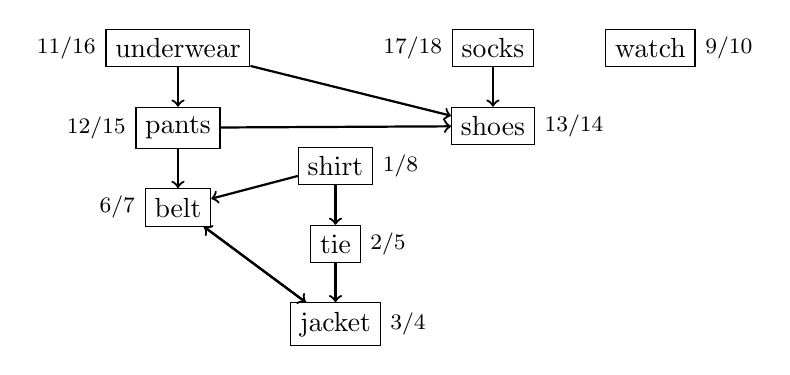
\begin{tikzpicture}[node distance=0.5cm and 0.8cm, every node/.style={draw}]
			\node[label=left:\footnotesize  11/16] (underwear) {underwear};
			\node[label=left:\footnotesize  12/15, below =of underwear] (pants) {pants};
			\node[label=left:\footnotesize  6/7, below =of pants] (belt) {belt};
			\node[label=right:\footnotesize 1/8] at (2, -1.5) (shirt) {shirt};
			\node[label=right:\footnotesize 2/5, below =of shirt] (tie) {tie};
			\node[label=right:\footnotesize 3/4, below =of tie] (jacket) {jacket};
			\node[label=left:\footnotesize  17/18] at (4,0) (socks) {socks};
			\node[label=right:\footnotesize 13/14, below =of socks] (shoes) {shoes};
			\node[label=right:\footnotesize 9/10] at (6,0) (watch) {watch};

			\foreach \from/\to in {
				underwear/pants, underwear/shoes, pants/shoes, socks/shoes,
				pants/belt, belt/jacket, shirt/belt, shirt/tie, tie/jacket, jacket/belt}
				\draw[->, thick] (\from) -- (\to);
		\end{tikzpicture}
		{\caption*{Directed graph of how to get ready in the morning with timestamps}}
	\end{figure}

	\begin{figure}[h]
		\centering
		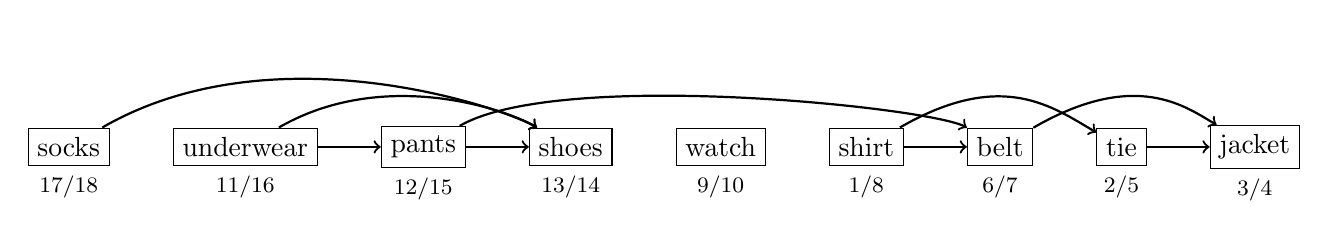
\begin{tikzpicture}[node distance=0.5cm and 0.8cm, every node/.style={draw}]
			\node[label=below:\footnotesize 17/18]  (socks) {socks};
			\node[label=below:\footnotesize 11/16, right =of socks] (underwear) {underwear};
			\node[label=below:\footnotesize 12/15, right =of underwear] (pants) {pants};
			\node[label=below:\footnotesize 13/14, right =of pants] (shoes) {shoes};
			\node[label=below:\footnotesize 9/10, right =of shoes] (watch) {watch};
			\node[label=below:\footnotesize 1/8, right =of watch] (shirt) {shirt};
			\node[label=below:\footnotesize 6/7, right =of shirt] (belt) {belt};
			\node[label=below:\footnotesize 2/5, right =of belt] (tie) {tie};
			\node[label=below:\footnotesize 3/4, right =of tie] (jacket) {jacket};
			\foreach \from/\to in {underwear/pants, pants/shoes,shirt/belt, tie/jacket}
				\draw[->, thick] (\from) -- (\to);
			\draw[->, thick] (socks)     .. controls +(30:3cm) and +(150:1cm) .. (shoes);
			\draw[->, thick] (underwear) .. controls +(30:2cm) and +(150:1cm) .. (shoes);
			\draw[->, thick] (shirt)     .. controls +(30:2cm) and +(150:1cm) .. (tie);
			\draw[->, thick] (belt)      .. controls +(30:2cm) and +(150:1cm) .. (jacket);
			\draw[->, thick] (pants)     .. controls +(30:2cm) and +(150:1cm) .. (belt);
		\end{tikzpicture}
		{\caption*{Topologically sorted so there's no conflicts}}
	\end{figure}



	%-----------------------------------------------------------------------------------------------------------------

	\subsection{Minimum Spanning Tree}
	\marginnote{\scriptsize{CLRS pg.625}}
	A Minimum Spanning Tree is a subgraph of a graph that contains all nodes and has lowest combined weight of all of it's edges. It's possible to have multiple Minimum Spanning Trees per graph, if the edge weights are not unique. We'll look at two algorithms to solve this problem.

	\begin{figure}[h]
		\centering
		\tikzstyle{vertex}=[draw,circle,minimum size=0.8cm]
		\tikzstyle{edge} = [draw,-]
		\tikzstyle{selected edge} = [draw,ultra thick,-]
		\begin{tikzpicture}[auto, swap]
			\foreach \pos/\name in {{(0,2)/a}, {(2,1)/b}, {(4,1)/c},
									{(0,0)/d}, {(3,0)/e}, {(2,-1)/f}, {(4,-1)/g}}
				\node[vertex] (\name) at \pos {$\name$};
			\foreach \source/ \dest /\weight in {b/a/7, c/b/8,d/a/5,d/b/9,
												 e/b/7, e/c/5,e/d/15,
												 f/d/6,f/e/8,
												 g/e/9,g/f/11}
				\path[edge] (\source) -- node {\scriptsize $\weight$} (\dest);
			\foreach \source / \dest in {d/a,d/f,a/b,b/e,e/c,e/g}
				\path [selected edge] (\source) -- (\dest);
		\end{tikzpicture}
		{\caption*{Minimum Spanning Tree of a weighted graph}}
	\end{figure}

	\subsubsection{Prim's Algorithm}
	\marginnote{\scriptsize{CLRS pg.634}}
	Prim's Alogithm is a {\bf Greedy Algorithm} using {\bf Priority Queues}. {\bf Avg. Case:} $O(E + V \log V)$ and best used for {\bf dense graphs}. At each step it grows the tree by one node, selecting the smallest edge available.

	\begin{lstlisting}[style=pseudo]
	PrimMST(G){
		add all nodes in G to Queue, Q with key = \infty
		while Q is not empty
			x = Q.extractMin()
			for all neighbours v of x
				if v is in Q and weight(x,v) < v.key
					v.parent = x
					v.key = weight(x,v)
	}
	\end{lstlisting}


	\subsubsection{Krushal's Algorithm}
	\marginnote{\scriptsize{CLRS pg.631}}
	Krushal's Algorithm is a {\bf Greedy Algorithm} using {\bf Disjoint Sets}. {\bf Avg. Case:} $O(E \log V)$ and best used for {\bf sparse graphs}. It first creates a set for each node and then a set of all edges ordered by weight. For each edge, if both nodes aren't in the same set together, it merges the sets together and adds that edge to the solution set. It ends when all nodes belong to a single set.

	\begin{lstlisting}[style=pseudo]
	KrushalMST(G){
		make Result an empty set
		make a set for each node that contains it
		foreach (u, v) in G.Edges ordered by weight(u, v)
			if Find-Set(u) != Find-Set(v)
				add (u,v) to Result
				Join-Sets(u, v)
		return Result
	}
	\end{lstlisting}


	%-----------------------------------------------------------------------------------------------------------------

	\subsection{Dijsktra's Algorithm}
	\marginnote{\scriptsize{CLRS pg.658}}

	Dijsktra's Algorithm finds the {\bf single-source shortest path} in a weighted graph. As Dijsktra's Algorithm tranverses the graph, it follows the path of lowest expected total distance. It keeps track of how good each branch is using a {\bf Min-Priority Queue}. {\bf Avg. Case:} $O(E + V \log V)$.
	\\ \\
	A greedy algorithm is used to choose the next node for each branch and will switch to a different branch if it no longer is the fastest. The variable $distance$ on each node in our code tracks the shortest path value to get to that node from the start.

	\begin{lstlisting}[style=pseudo]
	Dijsktra(G, start, goal){
		create Priority Queue Q
		add all nodes to Q with distance of \infty
		start.distance = 0
		while Q is not empty
			current = Q.extractMin()
			if current is goal
				goal.parent = current
				return ReconstructPath(goal, empty list)
			for each neighbour of current
				temp = current.distance + weight(current, neighbour)
				if temp < neighbour.distance
					neighbour.distance = temp
					neighbour.parent = current
	}
	ReconstructPath(node, result){
		if node has parent
			ReconstructPath(node.parent, result)
		result.push(node)
		return result
	}
	\end{lstlisting}


	%-----------------------------------------------------------------------------------------------------------------

	\subsection{A*}
	\marginnote{\scriptsize{CLRS pg.308}}
	The A* algorithm is a generalization of Dijkstra's algorithm that cuts down on the size of the subgraph that must be explored by using an additional {\bf heuristic} unique to the problem. The heuristic function helps guide the path in which the algorithm takes next. For example if the nodes have a coordinate location, the heuristic function could be the euclidean distance between the current node and the goal, making sure that the algorithm tries the closest branches first.
	\\ \\
	{\bf Avg. Case:} $O(\log h(x))$, where $h(x)$ is the optimal heuristic function.

	\begin{lstlisting}[style=pseudo]
	AStar(G, start, goal){
		create Priority Queue Q
		add all nodes to Q with score of \infty
		start.score = 0
		while Q is not empty
			current = Q.extractMin()
			if current is goal
				goal.parent = current
				return ReconstructPath(goal, empty list)
			for each neighbour of current
				temp = current.score + weight(current, neighbour) + heuristic(neighbor, goal)
				if temp < neighbour.score
					neighbour.score = temp
					neighbour.parent = current
	}
	ReconstructPath(node, result){
		if node has parent
			ReconstructPath(node.parent, result)
		result.push(node)
		return result
	}
	\end{lstlisting}


	%-----------------------------------------------------------------------------------------------------------------

	%-----------------------------------------------------------------------------------------------------------------

	\clearpage
	\subsection{Convex Hull}
	\marginnote{\scriptsize{CLRS pg.1029}}
	The Convex Hull of a set of points is the {\bf smallest polygon that contains all points}. Imagine it like an elastic band wrapped around a number of pegs in a board. {\bf Used with} bezier curves, pattern recogintion, image processing, statistics, and static code analysis. We'll look at two algorithms to solve this problem.

		\subsubsection{Graham's Scan}
		Graham's Scan starts at the lowest point in the set and iterates over the points in a counterclockwise direction, relative to this point. At each step it calculates the angle between the last two points and a the next point to try. If that angle is towards the left, we add the test point to our solution set. If that angle is to the right, we remove the last point from our solution set and repeat. {\bf Running time:} $O(n \log n)$.

		\begin{lstlisting}[style=pseudo]
		GScan(P){
			root = lowest point in P
			S = all points in P sorted by relative angle to root
			Hull = empty list

			Hull.push(root)
			Hull.push(S.pop())

			while S is not empty
				next = S.top()
				if angleDirection(Hull.secondLast(), Hull.last(), next) is left
					Hull.push(S.pop())
				else
					Hull.pop()
			return Hull
		}
		\end{lstlisting}

		\tikzstyle{point}=[circle,fill=black,minimum size=0.15cm,inner sep=0pt]
		\begin{figure}[h]
			\centering
			\begin{subfigure}{.4\textwidth}
				\centering
				\begin{tikzpicture}
					\node[point, label=below:\scriptsize p0] (p0) at (-1,-2) {};
					\foreach \pos/\name in {{(4,-1)/p1}, {(2,-1)/p2}, {(3,0)/p3}, {(4,1.5)/p4}, {(2,1)/p5}, {(0,0)/p6}, {(0,2)/p7}} {
						\node[point] (\name) at \pos {};
						\node[anchor=south west] at (\name) {\scriptsize \name};
					}
					\foreach \name in {p1,p2,p3,p4,p5,p6,p7}
						\path[draw, dotted, thick] (p0) -- (\name);

					\path[draw, ultra thick] (p0) -- (p1);
					\path[draw] (p1) -- (p2);

					\coordinate (b) at (-1,-2);
					\coordinate (c) at (4,-1);
					\coordinate (a) at (2,-1);
					\draw[fill=black!20] (c) -- ($(c)!8mm!(b)$) to[bend left] ($(c)!8mm!(a)$)  -- cycle;
				\end{tikzpicture}
				{\caption*{Add p2 to solution set, since $\angle$ p0 p1 p2 is facing left}}
			\end{subfigure}
			\begin{subfigure}{.4\textwidth}
				\centering
				\begin{tikzpicture}
					\coordinate (a) at (4,-1);
					\coordinate (c) at (2,-1);
					\coordinate (b) at (3,0);
					\draw[fill=black!20] (c) -- ($(c)!8mm!(b)$) to[bend left] ($(c)!8mm!(a)$)  -- cycle;

					\node[point, label=below:\scriptsize p0] (p0) at (-1,-2) {};
					\foreach \pos/\name in {{(4,-1)/p1}, {(2,-1)/p2}, {(3,0)/p3}, {(4,1.5)/p4}, {(2,1)/p5}, {(0,0)/p6}, {(0,2)/p7}} {
						\node[point] (\name) at \pos {};
						\node[anchor=south west] at (\name) {\scriptsize \name};
					}
					\foreach \name in {p1,p2,p3,p4,p5,p6,p7}
						\path[draw, dotted, thick] (p0) -- (\name);

					\path[draw, ultra thick] (p0) -- (p1);
					\path[draw, ultra thick] (p1) -- (p2);
					\path[draw] (p2) -- (p3);
				\end{tikzpicture}
				{\caption*{$\angle$p1 p2 p3 is facing right, remove p2}}
			\end{subfigure}
			\begin{subfigure}{.4\textwidth}
				\centering
				\begin{tikzpicture}
					\node[point, label=below:\scriptsize p0] (p0) at (-1,-2) {};
					\foreach \pos/\name in {{(4,-1)/p1}, {(2,-1)/p2}, {(3,0)/p3}, {(4,1.5)/p4}, {(2,1)/p5}, {(0,0)/p6}, {(0,2)/p7}} {
						\node[point] (\name) at \pos {};
						\node[anchor=south west] at (\name) {\scriptsize \name};
					}
					\foreach \name in {p1,p2,p3,p4,p5,p6,p7}
						\path[draw, dotted, thick] (p0) -- (\name);

					\path[draw, ultra thick] (p0) -- (p1);
					\path[draw] (p1) -- (p3);

					\coordinate (b) at (-1,-2);
					\coordinate (c) at (4,-1);
					\coordinate (a) at (3,0);
					\draw[fill=black!20] (c) -- ($(c)!8mm!(b)$) to[bend left] ($(c)!8mm!(a)$)  -- cycle;
				\end{tikzpicture}
				{\caption*{$\angle$p0 p1 p3 is good, so we add p3}}
			\end{subfigure}
			\begin{subfigure}{.4\textwidth}
				\centering
				\begin{tikzpicture}
					\coordinate (a) at (4,-1);
					\coordinate (c) at (3,0);
					\coordinate (b) at (4,1.5);
					\draw[fill=black!20] (c) -- ($(c)!8mm!(b)$) to[bend left] ($(c)!8mm!(a)$)  -- cycle;

					\node[point, label=below:\scriptsize p0] (p0) at (-1,-2) {};
					\foreach \pos/\name in {{(4,-1)/p1}, {(2,-1)/p2}, {(3,0)/p3}, {(4,1.5)/p4}, {(2,1)/p5}, {(0,0)/p6}, {(0,2)/p7}} {
						\node[point] (\name) at \pos {};
						\node[anchor=south west] at (\name) {\scriptsize \name};
					}
					\foreach \name in {p1,p2,p3,p4,p5,p6,p7}
						\path[draw, dotted, thick] (p0) -- (\name);

					\path[draw, ultra thick] (p0) -- (p1);
					\path[draw, ultra thick] (p1) -- (p3);
					\path[draw] (p3) -- (p4);
				\end{tikzpicture}
				{\caption*{$\angle$p1 p3 p4 is bad, remove p3}}
			\end{subfigure}
			\begin{subfigure}{.4\textwidth}
				\centering
				\begin{tikzpicture}
					\coordinate (b) at (4,-1);
					\coordinate (c) at (4,1.5);
					\coordinate (a) at (2,1);
					\draw[fill=black!20] (c) -- ($(c)!8mm!(b)$) to[bend left] ($(c)!8mm!(a)$)  -- cycle;
					\node[point, label=below:\scriptsize p0] (p0) at (-1,-2) {};
					\foreach \pos/\name in {{(4,-1)/p1}, {(2,-1)/p2}, {(3,0)/p3}, {(4,1.5)/p4}, {(2,1)/p5}, {(0,0)/p6}, {(0,2)/p7}} {
						\node[point] (\name) at \pos {};
						\node[anchor=south west] at (\name) {\scriptsize \name};
					}
					\foreach \name in {p1,p2,p3,p4,p5,p6,p7}
						\path[draw, dotted, thick] (p0) -- (\name);
					\path[draw, ultra thick] (p0) -- (p1);
					\path[draw, ultra thick] (p1) -- (p4);
					\path[draw] (p4) -- (p5);
				\end{tikzpicture}
				{\caption*{$\angle$p1 p4 p5 is good, add p4, etc.}}
			\end{subfigure}
			\begin{subfigure}{.4\textwidth}
				\centering
				\begin{tikzpicture}
					\node[point, label=below:\scriptsize p0] (p0) at (-1,-2) {};
					\foreach \pos/\name in {{(4,-1)/p1}, {(2,-1)/p2}, {(3,0)/p3}, {(4,1.5)/p4}, {(2,1)/p5}, {(0,0)/p6}, {(0,2)/p7}} {
						\node[point] (\name) at \pos {};
						\node[anchor=south west] at (\name) {\scriptsize \name};
					}

					\path[draw, ultra thick] (p0) -- (p1);
					\path[draw, ultra thick] (p1) -- (p4);
					\path[draw, ultra thick] (p4) -- (p7);
					\path[draw, ultra thick] (p7) -- (p0);
				\end{tikzpicture}
				{\caption*{Completed scan}}
			\end{subfigure}
		{\caption*{An example of Graham's Scan}}
	\end{figure}


		\clearpage

		\subsubsection{QuickHull}
		QuickHull is based off of QuickSort in that we use divide and conquer style. At each step we divide the current set by drawing a line between two points. For each side of the line we find the point farthest from the line, create a triangle between these three points. We remove all the points inside the triangle from the working set and repeat the same process on the two other triangle sides.
		\\ \\
		Just like QuickSort, QuickHull has a {\bf Avg Case}: $O(n \log n)$ and {\bf Worst Case}: $O(n^2)$.

		\begin{lstlisting}[style=pseudo]
		QuickHull(P){
			r = right most point in P
			l = left most point in P
			S = []
			S.push( (r,l) )
			while S is not empty
				(x,y) = S.pop()
				s = all points in P above line(x,y)
				if s is not empty
					p = point farthest from line(x,y) in s
					for each point r in triangle(x,y,p)
						remove r from P
					S.push( (x,p) )
					S.push( (p,y) )
			return P
		}
		\end{lstlisting}

		\tikzstyle{point}=[circle,fill=black,minimum size=0.15cm,inner sep=0pt]
		\tikzstyle{ignored point}=[circle,fill=black!30,minimum size=0.15cm,inner sep=0pt]
		\begin{figure}[h]
			\centering
			\begin{subfigure}[b][7cm][b]{.45\textwidth}
				\centering
				\begin{tikzpicture}
					\foreach \pos/\name in {{(0,2)/a},{(2,2.5)/b},{(4.5,1.5)/c},{(0,0)/d},{(3,0)/e},{(2,-1)/f},{(4,-1)/g},{(-1,-2)/h}}{
						\node[point] (\name) at \pos {};
						%\node[anchor=south west] at (\name) {\scriptsize \name};
					}
					\node[anchor=north east] at (h) {\large $x$};
					\node[anchor=south west] at (c) {\large $y$};
					\path[draw, thick] (h) -- (c);
				\end{tikzpicture}
				{\caption*{Find points x and y farthest to the right and left, and split the set of points}}
			\end{subfigure}
			\begin{subfigure}[b][7cm][b]{.45\textwidth}
				\centering
				\begin{tikzpicture}
					\foreach \pos/\name in {{(0,2)/a},{(2,2.5)/b},{(4.5,1.5)/c},{(0,0)/d},{(3,0)/e},{(2,-1)/f},{(4,-1)/g},{(-1,-2)/h}}{
						\node[point] (\name) at \pos {};
						%\node[anchor=south west] at (\name) {\scriptsize \name};
					}
					\node[anchor=north east] at (h) {\large $x$};
					\node[anchor=south west] at (c) {\large $y$};
					\path[draw, thick] (h) -- (c);
					\path[draw, dashed] (a) -- (1.75,-0.2500);
				\end{tikzpicture}
				{\caption*{Find the point farthest from line (x,y) on one side}}
			\end{subfigure}
			\begin{subfigure}[b][7cm][b]{.45\textwidth}
				\centering
				\begin{tikzpicture}
					\foreach \pos/\name in {{(0,2)/a}, {(2,2.5)/b}, {(4.5,1.5)/c}, {(3,0)/e}, {(2,-1)/f}, {(4,-1)/g}, {(-1,-2)/h}}
						\node[point] (\name) at \pos {};
					\foreach \pos/\name in {{(0,0)/d}}
						\node[ignored point] (\name) at \pos {};

					\node[anchor=north east] at (h) {\large $x$};
					\node[anchor=south east] at (a) {\large $a$};
					\node[anchor=south west] at (c) {\large $y$};
					\path[draw, thick] (h) -- (c);
					\path[draw, thick] (h) -- (a);
					\path[draw, thick] (a) -- (c);
				\end{tikzpicture}
				{\caption*{Create a triangle and remove all points from within it}}
			\end{subfigure}
			\begin{subfigure}[b][7cm][b]{.45\textwidth}
				\centering
				\begin{tikzpicture}
					\foreach \pos/\name in {{(0,2)/a}, {(2,2.5)/b}, {(4.5,1.5)/c}, {(3,0)/e}, {(2,-1)/f}, {(4,-1)/g}, {(-1,-2)/h}}
						\node[point] (\name) at \pos {};
					\foreach \pos/\name in {{(0,0)/d}}
						\node[ignored point] (\name) at \pos {};

						\node[anchor=north east] at (h) {\large $x$};
						\node[anchor=south east] at (a) {\large $a$};
						\node[anchor=south west] at (c) {\large $y$};
					\path[draw, thick] (h) -- (c);
					\path[draw, thick] (h) -- (a);
					\path[draw, thick] (a) -- (c);
					\path[draw, dashed] (b) -- (1.9,1.75);
				\end{tikzpicture}
				{\caption*{Repeat steps with line (x,a) and (a,y)}}
			\end{subfigure}
			\begin{subfigure}[b][7cm][b]{.45\textwidth}
				\centering
				\begin{tikzpicture}
					\foreach \pos/\name in {{(0,2)/a}, {(2,2.5)/b}, {(4.5,1.5)/c}, {(3,0)/e}, {(2,-1)/f}, {(4,-1)/g}, {(-1,-2)/h}}
						\node[point] (\name) at \pos {};
					\foreach \pos/\name in {{(0,0)/d}}
						\node[ignored point] (\name) at \pos {};

					\node[anchor=north east] at (h) {\large $x$};
					\node[anchor=south west] at (c) {\large $y$};
					\path[draw, thick] (h) -- (c);
					\path[draw, thick] (h) -- (a);
					\path[draw, thick] (a) -- (b);
					\path[draw, thick] (b) -- (c);
					\path[draw, dashed] (g) -- (2.75,0.4);
				\end{tikzpicture}
				{\caption*{Repeat the process with the other side of the line (x,y)}}
			\end{subfigure}
			\begin{subfigure}[b][7cm][b]{.45\textwidth}
				\centering
				\begin{tikzpicture}
					\foreach \pos/\name in {{(0,2)/a}, {(2,2.5)/b}, {(4.5,1.5)/c}, {(4,-1)/g}, {(-1,-2)/h}}
						\node[point] (\name) at \pos {};
					\foreach \pos/\name in {{(3,0)/e}, {(2,-1)/f}, {(0,0)/d}}
						\node[ignored point] (\name) at \pos {};

					\path[draw, thick] (h) -- (a);
					\path[draw, thick] (a) -- (b);
					\path[draw, thick] (b) -- (c);
					\path[draw, thick] (h) -- (g);
					\path[draw, thick] (g) -- (c);
				\end{tikzpicture}
				{\caption*{Completed scan}}
			\end{subfigure}
			{\caption*{An example of QuickHull}}
		\end{figure}


		\clearpage
		\subsection{k-Means Clustering}

		K-means clustering aims to partition a number of points in $k$ groups/clusters. We have the optiminal distribution of clusters when every point is closest to the center of it's cluster then any other center of the clusters. The problem is {\bf NP-hard}; however, there are efficient heuristic algorithm scan converge quickly to a local optimum. {\bf Used in} reducing an image color pallete to $k$ colors and feature analysis for machine learning.
		\\ \\
		As a heuristic algorithm, there is no guarantee that it will converge to the global optimum, and the result may depend on the initial clusters. As the algorithm is usually very fast, it is common to run it multiple times with different starting conditions. {\bf Worst Case:} $\Omega(2^n)$ to find globally optimal solution.
		\\ \\
		{\bf Method:} Choose $k$ "mean" points and place them randomly. Produce an {\bf Voronoi Diagram} using those "mean" points. Find the center of each region and move the "mean" point there. Repeat until the clusters settle. Run the algorithm multiple times with different initial "mean" points to assure the optimal solution is found.

		\tikzstyle{point}=[circle,fill=black!50,minimum size=0.15cm,inner sep=0pt]
		\tikzstyle{mpoint}=[fill=black,minimum size=0.15cm,inner sep=0pt]
		\begin{figure}[h]
			\centering
			\begin{subfigure}{.4\textwidth}
				\centering
				\begin{tikzpicture}[scale=0.4]
					\foreach \pos/\name in {{(0,7.5)/a1}, {(0,6.5)/b1}, {(0,5.5)/c1},
											{(1,4)/a2}, {(1,3)/b2}, {(2,2)/c2}, {(3,2)/d2}, {(4,3)/e2}, {(4,4)/f2},
											{(5,7.5)/a3}, {(5,6.5)/b3}, {(5,5.5)/c3}}
						\node[point] (\name) at \pos {};

					\node[mpoint] (m1) at (0.75,8.5) {};
					\node[mpoint] (m2) at (0.75,4.5) {};
					\node[mpoint] (m3) at (4.75,4.5) {};
				\end{tikzpicture}
				{\caption*{Place three mean points randomly}}
			\end{subfigure}
			\begin{subfigure}{.4\textwidth}
				\centering
				\begin{tikzpicture}[scale=0.4]
					\foreach \pos/\name in {{(0,7.5)/a1}, {(0,6.5)/b1}, {(0,5.5)/c1},
											{(1,4)/a2}, {(1,3)/b2}, {(2,2)/c2}, {(3,2)/d2}, {(4,3)/e2}, {(4,4)/f2},
											{(5,7.5)/a3}, {(5,6.5)/b3}, {(5,5.5)/c3}}
						\node[point] (\name) at \pos {};

					\node[mpoint] (m1) at (0.75,8.5) {};
					\node[mpoint] (m2) at (0.75,4.5) {};
					\node[mpoint] (m3) at (4.75,4.5) {};

					\path[draw] (3.5,7) -- (-1,7);
					\path[draw] (3.5,7) -- (3.5,1);
					\path[draw] (3.5,7) -- (5.5,9);
				\end{tikzpicture}
				{\caption*{Create regions based on the mean points}}
			\end{subfigure}
			\begin{subfigure}{.4\textwidth}
				\centering
				\begin{tikzpicture}[scale=0.4]
					\foreach \pos/\name in {{(0,7.5)/a1}, {(0,6.5)/b1}, {(0,5.5)/c1},
											{(1,4)/a2}, {(1,3)/b2}, {(2,2)/c2}, {(3,2)/d2}, {(4,3)/e2}, {(4,4)/f2},
											{(5,7.5)/a3}, {(5,6.5)/b3}, {(5,5.5)/c3}}
						\node[point] (\name) at \pos {};
					\node[mpoint, fill=black!50] (m1o) at (0.75,8.5) {};
					\node[mpoint, fill=black!50] (m2o) at (0.75,4.5) {};
					\node[mpoint, fill=black!50] (m3o) at (4.75,4.5) {};

					\node[mpoint] (m1) at (0,7.5) {};
					\node[mpoint] (m2) at (1.15,3.6) {};
					\node[mpoint] (m3) at (4.5,5.6) {};

					\path[draw, ->] (m1o) -- (m1);
					\path[draw, ->] (m2o) -- (m2);
					\path[draw, ->] (m3o) -- (m3);

					\path[draw] (3.5,7) -- (-1,7);
					\path[draw] (3.5,7) -- (3.5,1);
					\path[draw] (3.5,7) -- (5.5,9);
				\end{tikzpicture}
				{\caption*{Find the center of the points in each region and move the mean points there}}
			\end{subfigure}
			\begin{subfigure}{.4\textwidth}
				\centering
				\begin{tikzpicture}[scale=0.4]
					\foreach \pos/\name in {{(0,7.5)/a1}, {(0,6.5)/b1}, {(0,5.5)/c1},
											{(1,4)/a2}, {(1,3)/b2}, {(2,2)/c2}, {(3,2)/d2}, {(4,3)/e2}, {(4,4)/f2},
											{(5,7.5)/a3}, {(5,6.5)/b3}, {(5,5.5)/c3}}
						\node[point] (\name) at \pos {};

					\node[mpoint] (m1) at (0,7.5) {};
					\node[mpoint] (m2) at (1.15,3.6) {};
					\node[mpoint] (m3) at (4.5,5.6) {};

					\path[draw] (2.25,6) -- (-1,4);
					\path[draw] (2.25,6) -- (4.25,1);
					\path[draw] (2.25,6) -- (4,8.5);
				\end{tikzpicture}
				{\caption*{Re-draw the Voronoi Diagrams using the mean points and repeat}}
			\end{subfigure}

		\end{figure}



\clearpage
\section{Dynamic Programming}
	Dynamic Programming is a technique for solving difficult problems by breaking them down into simpler subproblems. The goal is to find and utilize {\bf overlapping subproblems} to limit the solution space. Two main methods are used:
	\begin{description}
		\item[Top-down] Starts at the "top" of the problem, splitting it into subprolema nd solving them recursively. Whenever a solution is found, it's recorded. If that subproblem is ever visited in the recursion, the previously solved answer is used. {\bf Examples} Fibonacci Numbers.
		\item[Bottom-up] Topologically progress through the problem, starting at the lowest base cases. This ensures only the paths needed are considered. This process may span mutliple dimensions of the problem, leading to a tabular lookup table. {\bf Examples:} The knapsack problem,
	\end{description}

	\subsection{Problems}
		\begin{enumerate}
			\item A child is running up a staircase with n steps, and can hop either 1 step, 2 steps, or 3 steps at a time. Implement a method to count how many possible ways the child can run up the stairs.
			\item Write a method to compute all permutations of a string.
			\item Write an algorithm to print all ways of arranging eight queens on an 8x8 chess board so that none of them share the same row, column or diagonal. In this case, "diagonal" means all diagonals, not just the two that bisect the board.
		\end{enumerate}


\clearpage
\section{Systems}
	\subsection{Scheduling}

		turn around time,
		response time
		multi-level feedback queue
		cache affinity
		cache coherence
		MQMs


	\subsection{Threads}

	address space


	A thread's {\bf critical section} is the part of the code where the thread wishes to access memory shared by other threads. Two threads both interacting the sma epiece of shared memory at the same time can have unexpected results.

	A mutex (mutual exclusion) ensures the two threads/processes are not in their critical sections at the same time. Mutexes can be obtained using locks, conditional variables, or semaphores.


	\subsection{Locks}


	\subsection{Condition Variables}
	In multi-threaded programs it's useful for a thread to wait until a certain condition is met, not just if something has been unlocked. It is a {\bf queue} that threads can put themselves in until the variable becomes 0.

	A condition avriable has two operations; \texttt{wait()} and \texttt{signal()}. \texttt{wait()} is used to put the thread to sleep and wait for the signal

	bounded buffer problem




	\subsection{Semaphores}
		A semaphore is an abstract data type used for controlling access between multiple processes running in parallel. {\bf Counting Semaphores} allow for an internal count, where as {\bf Binary Semaphores} are restricted to 1/0, useful for simple locks. The value of the semaphore is the number of units of the resource that are currently available.

		\begin{lstlisting}[style=pseudo]
	class semaphore{
		init(v){
			semaphore's value is set to v
		}
		wait(){
			wait until value of semaphore is greater than 0
			decrement the value of semaphore by 1
		}
		post(){
			increment the value of semaphore by 1
			if there are 1 or more threads waiting, wake 1
		}
	}
		\end{lstlisting}

		To build a {\bf simple lock}, we can use a binary semaphore and just surround the critical section
		\begin{lstlisting}[style=pseudo]
	s = new Semaphore(0, 1)
	s.wait()
	//critical section
	s.post()
		\end{lstlisting}

		To use a semaphore a {\bf condition variable} For example a thread waiting until a list is empty.

		\begin{lstlisting}[style=pseudo]
	s = new Semaphore(0,0)
	parent(){
		start child
		s.wait()
		return "finished"
	}
	child(){
		do action
		s.post()
		return
	}
		\end{lstlisting}




	\subsection{Deadlocks}
		In order for a deadlock to occur, you must have all four of the following conditions met:
		\begin{enumerate}
			\item {\bf Mutual Exclusion}: Only one process can access a resource at a given time. (Or, more accurately, there is limited access to a resource. A deadlock could also occur if a resource has limited quantity.)
			\item {\bf Hold and Wait}: Processes already holding a resource can request additional resources, without relinquishing their current resources.
			\item {\bf Wo Preemption}: One process cannot forcibly remove another process'resource.
			\item {\bf Circular Wait}: Two or more processes form a circular chain where each process is waiting on another resource in the chain.
		\end{enumerate}




	\subsection{Problems}
		\begin{enumerate}
			\item Design a class which provides a lock only if there are no possible deadlocks.
			\item In the famous dining philosophers problem, a bunch of philosophers are sitting around a circular table with one chopstick between each of them. A philosopher needs both chopsticks to eat, and always picks up the left chopstick before the right one. A deadlock could potentially occur if all the philosophers reached for the left chopstick at the same time. Using threads and locks, implement a simulation of the dining philosophers problem that prevents deadlocks.
		\end{enumerate}

\clearpage
\section{Cryptography}
	\subsection{Assymetric Cryptosystems}
		RSA is one of the first practical assymeteric cryptosystems and is widely used to secure data currently. Not only does it encrypt data from being read by the wrong party, but it also verifies that the data came from the intended sender. It does this by using a {\bf Public and Private Key Encryption}.

		\subsubsection{Key Generation}
			\begin{enumerate}
				\item Choose two distinct prime numbers $p$ and $q$, where $n = pq$ \hfill \\
					\small{$\phantom{\rightarrow} p = 61, q = 53, n = 61 \times 53 = 3233$}
				\item $\phi(n) = (p - 1)(q - 1)$, where $\phi$ is Euler's totient function. \hfill \\
					\small{$\phantom{\rightarrow} \phi(3233) = (61 - 1)(53 - 1) = 3120$}
				\item Choose an integer $public$ such that $gcd(public, \phi(n)) = 1$, therefore $public$ and $\phi(n)$ are coprime. \hfill \\
					\small{$\phantom{\rightarrow} public = 17$}
				\item Determine $private$ as $private^{-1} \equiv public \bmod{\phi(n)}$, therefore $private$ is the modular multiplicative inverse of $public \bmod{\phi(n)}$ \hfill \\
					\small{$\phantom{\rightarrow} private = 2753$}
			\end{enumerate}
			{\bf Encryption} of message $M$ is done by $c = M^{public} \bmod{n}$, where $c$ is the ciphertext.
			\begin{equation}
				\textbf{encrypt}(M) = M^{17} \bmod{3233} = c
			\end{equation}
			{\bf Decryption} of $c$ is done by $M = c^{private} \bmod{n}$.
			\begin{equation}
				\textbf{decrypt}(c) = c^{2753} \bmod{3233} = M
			\end{equation}

		\subsubsection{Sending Messages}
		Bob wants to send a secure message $M$ to Alice. Not only is Bob worried about someone else reading the message, but other people may pretend to be him and send messages as him to Alice. They agree to use RSA and both create a public and private key for themselves. They share their publics keys with eachother and keep their private keys a secret. This is how Bob would prepare his message.
		\begin{figure}[h]
			\centering
			\begin{enumerate}
				\item Ensures only Alice can open it \hfill \\
					$\textbf{encrypt}(M, public_{alice}) = c_1$
				\item Ensures only Bob could have sent it \hfill \\
					$\textbf{encrypt}(c_1, private_{bob}) = c_2$
			\end{enumerate}
			{\caption*{Bob prepares his message to Alice}}
		\end{figure}

		\begin{figure}[h]
			\centering
			\begin{enumerate}
				\item Verifies that Bob sent it \hfill \\
					$\textbf{decrypt}(c_2, public_{bob}) = c_1$
				\item Opens it with her private key \hfill \\
					$\textbf{decrypt}(c_1, private_{alice}) = M$
			\end{enumerate}
			{\caption*{Alice opens her message}}
		\end{figure}

	\subsection{Cryptographic Hash Functions}
		A cryptographic hash function is a hash function that takes data of arbitrary size and returns a fixed-size bit string. The ideal cryptographic hash function has four main properties:
		\begin{description}
			\item[Ease]: Easy to compute the hash value for any given message
			\item[One-way]: Can not generate a message from a hash
			\item[Avalanche]: Small changes in the data drastically change the hash
			\item[Collision Resistant]: Infeasible to find two different messages with the same hash.
		\end{description}
		{\bf Used as} digital signatures, for data fingerprinting, to detect duplicate data or uniquely identify files, and as checksums to detect accidental data corruption. We'll look at two common cryptographic hash functions.


		\begin{figure}[h]
			\centering
			\tikzstyle{input}=[draw, minimum width=2.5cm, minimum height=1cm, align=center]
			\tikzstyle{md5}=[draw, minimum width=2.5cm, minimum height=1cm, align=center,font=\ttfamily\scriptsize]
			\tikzstyle{sha2}=[draw, minimum width=5cm, minimum height=1cm, align=center,font=\ttfamily\scriptsize]
			\begin{tikzpicture}[node distance=0.3cm]
				\node[md5] (ax) {C78A 8D63 2B6E 324F \\ 8D3C A872 935E 47EC};
				\node[md5, below =of ax] (bx) {2E60 96AE D8F7 FDB2 \\ 4103 077C D1E5 558F};
				\node[md5, below =of bx] (cx) {6AA2 1745 9FCB DA60 \\ 11C3 1E7A ED87 DBB2};

				\node[input, left =of ax] (a) {Look out!};
				\node[input, left =of bx] (b) {A man-eating \\ chicken};
				\node[input, left =of cx] (c) {A man eating \\ chicken};

				\node[above =of ax] (n2) {MD5 Hash};
				\node[above =of a] (n1) {Input};

				\path[draw, ->] (a) -- (ax);
				\path[draw, ->] (b) -- (bx);
				\path[draw, ->] (c) -- (cx);
			\end{tikzpicture}
			\hspace{1cm}
			\begin{tikzpicture}[node distance=0.3cm]
				\node[sha2] (ax) {9469 D02A 2A9A 5634 9746 3542 00E9 0D0A \\ F725 399D 7E40 098A 4AFC 5585 80CE 56F6};
				\node[sha2, below =of ax] (bx) {5FB5 D353 E67C 176D 7A02 DEA1 6900 8FB6 \\ 09D4 0EB4 5AFF A831 9BEE FD33 A416 9C8E};
				\node[sha2, below =of bx] (cx) {5F08 2191 4418 CE2B 1ADD D090 D8ED 85C0 \\ 89A0 68D5 B347 FFE3 0770 5AD3 62E2 7EC6};

				\node[input, left =of ax] (a) {Look out!};
				\node[input, left =of bx] (b) {A man-eating \\ chicken};
				\node[input, left =of cx] (c) {A man eating \\ chicken};

				\node[above =of ax] (n2) {SHA256 Hash};
				\node[above =of a] (n1) {Input};

				\path[draw, ->] (a) -- (ax);
				\path[draw, ->] (b) -- (bx);
				\path[draw, ->] (c) -- (cx);
			\end{tikzpicture}
			{\caption*{Notice that small changes in the input cause the hash to change significantly; Avalanche effect}}
		\end{figure}



		\subsubsection{MD5}
		MD5 produces a 128-bit hash value, usually expressed as a 32 digit hexadecimal number. It is {\bf not collision resistant}, making it not suitable for security applications, like SSL certificates or digital signatures. {\bf Used mostly} to verify message integrity when transmitting data.
		\\ \\
		{\bf Method:} The MD5 hash algorithm is broken down into 4 rounds of 16 operations. These operations manipulate four 32-bit words, $A$, $B$, $C$, and $D$, which are initialize with default values. Each round uses a different function on words $B$, $C$, and $D$, which then get mixed with a 32-bit block of the input data and a 32-bit constant. That result is then left bit rotated and stored in word $A$. All words get rotated by one position ($A \rightarrow B$) and the process is repeated.

		\subsubsection{SHA-2}
		SHA-2 comes in two variants, that produce 256 and 512 bit hash values. SHA-2 belongs to the family of hash algorithms; SHA-0, SHA-1, SHA-2, and SHA-3. Security flaws were discovered in SHA-1, leading to SHA-2's widespread adoption. {\bf Used in} security applications and protocols, including TLS and SSL, PGP, SSH, S/MIME, Bitcoin and IPsec.


	\subsection{Security Attacks}
		If we wanted to store private information, such as user's password, one technique we could use is to keep a hash of the user's password, rather than storing it directly. This prevents leaking of your user's passwords, since the hash can only be used to verify. We'll look at a few methods people use to bypass/break a system like this.

		\subsubsection{Brute-force Attack}
		A Brute-force attack consists of systematically checking all possible keys or passwords until the correct one is found. In the worst case, this would involve traversing the entire search space. Longer keys are exponentially more difficult to break then shorter ones. A cipher with $n$ bits has a worst-case of $2^n$. Breaking a symmetric 256-bit key by brute force requires $2^{128}$ times more computational power than a 128-bit key. 50 supercomputers that could check a billion billion ($10^{18}$) keys per second, would require about $30^{51}$ years to exhaust the 256-bit key space.
		\\ \\
		{\bf To counter} a brute-force attack you can limit the number of attempts that a passphrase can be tried, by introducing time delays between successive attempts, or by increasing the attempt's complexity by requiring a CAPTCHA or a second-step verification.

		\subsubsection{Dictionary Attack}
		A Dictionary Attack is similar to Brute-force, but take advantage of the fact that most people use shorter passpharse that uses a common set of words with slight variation, such as appending a digit, eg. {\it 'password1'}. They are not guaranteed to succeed, and can be easily {\bf countered} by including random characters within the passpharse, sppliting up common words, or simply by increasing the length of your passphrase.

		\subsubsection{Rainbow Tables}
		A Rainbow Table is a {\bf pre-computed} look-up table for reversing cryptographic hash functions. Before an attack a rainbow table will be created by exploring the passphrase solution space and saving it's corresponding hash. There are {\bf space vs. time trade-offs} as the possible passphrase solution space could be very large, so Rainbow Tables don't map it entirely. Using techniques from a Dictionary-Attack, you could create a Rainbow Table of very common passpharses to quickly reverse those. You can use a "salt" in your hash to {\bf counter} a Rainbow tables, as it makes the solution space infeasibly big.
		\begin{lstlisting}[style=pseudo, basicstyle={\footnotesize\ttfamily}]
	Searching for hash(apple) in users' hash list... : Matches [alice3, 0bob0, charles8]
	Searching for hash(blueberry) in users' hash list... : Matches [usr10101, timmy, john91]
	Searching for hash(letmein) in users' hash list... : Matches [wilson10, dragonslayerX, joe1984]
	Searching for hash(s3cr3t) in users' hash list... : Matches [bruce19, knuth1337, john87]
	Searching for hash(z@29hjja) in users' hash list... : No users used this password
		\end{lstlisting}

		\subsubsection{Hash Salting}
		Rainbow tables only work because each password is hashed the exact same way. If two users have the same password, they'll have the same password hashes. We can prevent these attacks by randomizing each hash, so that when the same password is hashed twice, the hashes are not the same. To counter this we generate a new random string of characters called a "salt" each time we save a password . We append the salt to the password, hash it, and store the result with the salt for that user. To verify a password, we lookup the salt, append it to the password, hash it and match it to what we have stored.
		\begin{lstlisting}[style=pseudo, basicstyle={\footnotesize\ttfamily}]
	hash("hello")                        = 2cf24dba5fb0a30e26e83b2ac5b9e29e1b161e5c1fa7425e73043362938b9824
	hash("hello" + "QxLUF1bgIAdeQX") = 9e209040c863f84a31e719795b2577523954739fe5ed3b58a75cff2127075ed1
	hash("hello" + "bv5PehSMfV11Cd") = d1d3ec2e6f20fd420d50e2642992841d8338a314b8ea157c9e18477aaef226ab
	hash("hello" + "YYLmfY6IehjZMQ") = a49670c3c18b9e079b9cfaf51634f563dc8ae3070db2c4a8544305df1b60f007
		\end{lstlisting}




\clearpage
\section{Behavourial Questions}
	\subsection{Project Questions}
		You will most likely be ask at least one of the following questions below. Prep a response for each question specifying a related project/job.
		\begin{itemize}
			\item Mosting Challenging
			\item Most Challenging
			\item What You Learned
			\item Most Interesting
			\item Hardest Bug
			\item Enjoyed Most
			\item Conflicts with Teammates
		\end{itemize}
		Also, for each item on your resume; Project, job, qualification, etc. you should have a fun story or justification for it. Remember to structure your story to have a {\bf one sentence hook} and a {\bf brief} explanation. Memorize a few keywords for each, and build your story from that.

	\subsection{Weaknesses}
		When asked about your weaknesses, {\bf give a real weakness}. "My greatest weakness is that I work too hard" is a cop-put and they'll see right through it. A better answer conveys a real, legitimate weakness but emphasizes how you work to overcome it. Ask a close friend/co-worker to give you a honest answer for this.
		\\ \\
		{\bf For example:} "Sometimes, I don't have a very good attention to detail. While that's good because it lets me execute quickly, it also means that I sometimes make careless mistakes. Because of that, I make sure to always have someone else double check my work.""

	\subsection{Questions for Your Interviewer}
		Questions you ask your interviewer will factor in their decisions, whether subconsciously or consciously. Prepare them in advance.

		\subsubsection{Genuine Questions}
			These questions will give you a good feel for what the day-to-day life is like at the company.
			\begin{enumerate}
				\item "How much of your day do you spend coding?"
				\item "How many meetings do you have every week?"
				\item "What is the ratio of testers to developers to program managers? What is the interaction like? How does project planning happen on the team?"
			\end{enumerate}

		\subsubsection{Insightful Questions}
			These questions are designed to demonstrate your deep knowledge of programming or technologies, and they also demonstrate your passion for the company or product.
			\begin{enumerate}
				\item "I noticed that you use technology X. How do you handle problem Y?"
				\item "Why did the product choose to use the X protocol over the Y protocol? I know it has benefits like A, B, C, but many companies choose not to use it because of issue D."
			\end{enumerate}

		\subsubsection{Passion Questions}
			These questions are designed to demonstrate your passion for technology. They show that you're interested in learning and will be a strong contributor to the company.
			\begin{enumerate}
				\item "I'm very interested in scalability. Did you come in with a background in this, or what opportunities are there to learn about it?"
				\item "I'm not familiar with technology X, but it sounds like a very interesting solution. Could you tell me a bit more about how it works?""
			\end{enumerate}


\clearpage
\section{Designing Algorithms}
	Quickly designing algorithms in interviews can be tough. The following are techniques that will help you.

	\subsection{Five Algorithm Approaches}
		The following are five techniques for quickly figuring out an algorithm for a solution.

		\begin{description}
			\item[Examplify] Create multiple examples of the problem and try to find a pattern. \par
				%\textit{Example: Given a time, calculate the angle between the hour and minute hand} \par
				%Draw a few examples, figure out the angle between the hour/minute hand and 12:00, then make a formula.
			\item[Pattern Matching] Find what problems the algorithm is similar to and modify them. \par
				%\textit{Example: A sorted array has been rotated so that the elements might appear in the order 3456712. How would you find the minimum element?} \par
				%Two problems that are similar; 1) Find the minimum element in an array, 2) Find a particular element in a sorted array (i.e., binary search)

			\item[Simplify and Generalize] Change the contraints of the problem to make it simplier and solve it. USe the solution to create a more generalized apporach. \par
				%\textit{Example: A ransom note can be formed by cutting words out of a magazine to form a new sentence. How would you figure out if a ransom note (represented as a string) can be formed from a given magazine (string)?} \par
				%Start with cutting out just characters, then generalize to words.

			\item[Base Case and Build] Solve the problem for a few base cases (n = 1,2,3), then build a solution for $n$ where we know the solution for $n - 1$.
			\item[Data Structure Brainstorm] Run through your list of data structures and try to apply each one until one fits.
		\end{description}


	\subsection{Design Patterns}
		There are {\bf many} design patterns that have much material written about them. We will only cover the most used ones.
		\begin{description}
			\item[Observer] Is an object that maintains a list of dependants called observers and notifies the of any state changes, usually by calling methods. {\bf Used in} event handling systems.

			\item[Singleton] A class has only one instance and ensures access to the instance through the application. Often used for {\bf state objects}. \par
				\begin{lstlisting}[style=pseudo]
	class State {
		_instance = null;
		getlnstance(){
			if (_instance == null)
				_instance = new State();
			return _instance;
		}
	}
				\end{lstlisting}

			\item[Wrapper] Is used to provide a simplifed and expected interface to a larger, more complex object. It also {\bf decouples the code} that uses the system from the details of the subsystems, making it easier to modify the system later. Also known as {\bf Facade, Adpater, or Decorater}.

			\item[Factory] An interface for creating an instance of a class. Creating an object often requires more coplex processes that are not needed once the   object is created. A factory can contain these processes to keep the object's definition cleaner. Can also produce {\bf multiple types} of objcts. \par
				\begin{lstlisting}[style=pseudo]
	class CardGame {
		createCardGame(type) {
			if type == GameType.Poker
				return new PokerGame()
			else if type == GameType.BlackJack
				return new BlackJackGame()
			return null;
		}
	}
				\end{lstlisting}

		\end{description}


	\subsection{Object-Oriented Design}
		Regardless of whether the object is a physical item or a technical task, object-oriented design questions can be tackled in similar ways. The following approach will work well for many problems.
		\begin{enumerate}
			\item {\bf Handle Ambigulty} Object-oriented design (OOD) questions are often intentionally vague in order to test whether you'll make assumptions or if you'll ask clarifying questions. You should inquire who is going to use it and how they are going to use it. Depending on the question, you may even want to go through the "six Ws": who, what, where, when, how, why.
			\item {\bf Define the Core Objects} Figure out the key things you are going to create objects for.
			\item {\bf Analyze Relationships} Decide how your core objects interact with each. Which objects are members of which other objects? Do any objects inherit from any others? Are relationships many-to-many or one-to-many? It's very easy to make incorrect assumptions. You should talk to your interviewer about how general purpose your design should be.
			\item {\bf Investigate Actions} Identify what actions/methods each object will want to have and how they will effect their relationship with other objects.
	\end{enumerate}

	\subsection{Testing}
		Consider the following types of test cases when testing your alogrithms.
		\begin{description}
			\item[The Normal Case] Does it generate the correct output for typical inputs? Remember to think about potential issues here. For example, because sorting often requires some sort of partitioning, it's reasonable to think that the algorithm might fail on arrays with an odd number of elements, since they can't be evenly partitioned. Your test case should list both examples.
			\item[The Extremes] What happens when you pass in an empty array? Or a very small (one element) array? What if you pass in a very large one?
			\item[Nulls and "Illegal" Input] It is worthwhile to think about how the code should behave when given illegal input. For example, if you're testing a function to generate the nth Fibonacci number, your test cases should probably include the situation where n is negative.
			\item[Strange Input] What happens when you pass in an already sorted array? Or an array that's sorted in reverse order?
		\end{description}

	\subsection{Problems}
		\begin{enumerate}
			\item Design the data structures for a generic deck of cards. Explain how you would subclass the data structures to implement blackjack.
			\item Design a parking lot using object-oriented principles.
			\item Explain how you would design a chat server. In particular, provide details about the various backend components, classes, and methods. What would be the hardest problems to solve.
			\item Design and implement a hash table which uses chaining (linked lists) to handle collisions.
			\item How would you test an ATM in a distributed banking system?
		\end{enumerate}

%
%
		%\clearpage
		%\section{Web}
			%\subsection{SSL and HTTPS}
			%\subsection{EcmaScript 5}
			%\subsection{AJAX}
			%\subsection{Web RPC}
			%\subsection{Full Request}
				%%https://github.com/alex/what-happens-when
%
		%\clearpage
		%\section{Big Data}
			%\subsection{Hadoop}
			%\subsection{Databases?}
			%\subsection{MapReduce}



\end{document}